% **************************************************************************************************************
% A Classic Thesis Style
% An Homage to The Elements of Typographic Style
%
% Copyright (C) 2011 Andr\'e Miede http://www.miede.de
%
% If you like the style then I would appreciate a postcard. My address
% can be found in the file ClassicThesis.pdf. A collection of the
% postcards I received so far is available online at
% http://postcards.miede.de
%
% License:
% This program is free software; you can redistribute it and/or modify
% it under the terms of the GNU General Public License as published by
% the Free Software Foundation; either version 2 of the License, or
% (at your option) any later version.
%
% This program is distributed in the hope that it will be useful,
% but WITHOUT ANY WARRANTY; without even the implied warranty of
% MERCHANTABILITY or FITNESS FOR A PARTICULAR PURPOSE.  See the
% GNU General Public License for more details.
%
% You should have received a copy of the GNU General Public License
% along with this program; see the file COPYING.  If not, write to
% the Free Software Foundation, Inc., 59 Temple Place - Suite 330,
% Boston, MA 02111-1307, USA.
%
% **************************************************************************************************************
% Note:
%    * You must not use "u etc. in strings/commands that will be spaced out (use \"u or real umlauts instead)
%    * New enumeration (small caps): \begin{aenumerate} \end{aenumerate}
%    * For margin notes: \graffito{}
%    * Do not use bold fonts in this style, it is designed around them
%    * Use tables as in the examples
%    * See classicthesis-ldpkg.sty for useful commands
% **************************************************************************************************************
% To Do:
%		 * [high] Check this out: http://www.golatex.de/koma-script-warnung-in-verbindung-mit-listings-package-t2058.html
%    * [medium] mathbb in section-titles/chapter-titles => disappears somehow in headlines!!!
%    * [low] Calculate text block size for Libertine font
%    * [low] Think about processing a4paper, a5paper, 10pt, 11pt, 12pt etc. options for typearea layout
%            (store values in internal variables and handle by \AtEndOfPackage{\areaset...})
% **************************************************************************************************************
\documentclass[ twoside,openright,titlepage,fleqn,numbers=noenddot,headinclude,%1headlines,% letterpaper a4paper
                11pt,a4paper,BCOR5mm,footinclude=true,cleardoublepage=empty,abstractoff % <--- obsolete, remove (todo)
                ]{scrreprt}

% ********************************************************************
% Development Stuff
% ********************************************************************
\listfiles
%\usepackage[l2tabu, orthodox, abort]{nag}
%\usepackage[warning, all]{onlyamsmath}
% ********************************************************************
% Re-usable information
% ********************************************************************
\newcommand{\myTitle}{The effect of Orientation time on the perceived efficiency of smartphone authentication mechanisms}
\newcommand{\myDegree}{Bachelor Thesis\xspace}
\newcommand{\myName}{Serin Bazzi\xspace}
\newcommand{\myProf}{Dr. Emanuel von Zezschwitz\xspace}
\newcommand{\myOtherProf}{Prof. Dr. Matthew Smith\xspace}
\newcommand{\mySupervisor}{Christian Tiefenau, M. Sc.\xspace}
\newcommand{\myDepartment}{Institute of Computer Science 4\xspace}
\newcommand{\myFaculty}{Methods in Multi-Layer Usable Security Research\xspace}
\newcommand{\myUni}{\protect{Rheinische Friedrich-Wilhelms-Universit\"{a}t Bonn }\xspace}
\newcommand{\myLocation}{Bonn\xspace}
\newcommand{\myTime}{January 10th 2020\xspace}
\newcommand{\myVersion}{1.0\xspace}
%*******************************************************
% Packages with options that might require adjustments
%*******************************************************
\usepackage[latin1]{inputenc}
\usepackage[ngerman,american]{babel}
\usepackage[square,numbers]{natbib}
\usepackage{algorithm}
\usepackage{algorithmic}
\usepackage{multirow}
\usepackage{verbatim}
\usepackage[absolute]{textpos}
\usepackage{amsthm}
\newtheorem{definition}{Definition}
\usepackage[fleqn]{amsmath} % math environments and more by the AMS
%\usepackage{varioref} % load BEFORE classicthesis-ldpkg
%*******************************************************
\usepackage{classicthesis-ldpkg} % [backref]
%*******************************************************
% Options for classicthesis.sty:
% tocaligned eulerchapternumbers drafting linedheaders listings
% subfig nochapters beramono eulermath parts minionpro pdfspacing
% dottedtoc minionprospacing manychapters floatperchapter
\usepackage[eulerchapternumbers,listings,%drafting,%linedheaders,%pdfspacing,%listings,
						subfig,eulermath,parts,dottedtoc,floatperchapter]{classicthesis}%

% Change these parameters in order to resize the text area on each page
\areaset[12mm]{15cm}{761pt}%{312pt}{761pt} % Width and height of text
           \setlength{\marginparwidth}{3em}%{7em}% Width of margin
           \setlength{\marginparsep}{2em}% Distance between text and margin

%
% Use "my_enumerate" instead of "enumerate" in order to produce enumerations without vertical space between items
%
\newenvironment{my_enumerate}{
\begin{enumerate}
  \setlength{\itemsep}{1pt}
  \setlength{\parskip}{0pt}
  \setlength{\parsep}{0pt}}{\end{enumerate}
}

%*******************************************************
% Some font experiments
%*******************************************************
%\usepackage[osf]{libertine}
%\usepackage{hfoldsty}
%\usepackage[light,condensed,math]{iwona}
%\renewcommand{\sfdefault}{iwona}
%\usepackage{lmodern} % <-- no osf support :-(
%\usepackage[urw-garamond]{mathdesign} <-- no osf support :-(

%*******************************************************
% Fine-tuning for the text area
%*******************************************************
%\linespread{1.05} % a bit more for Palatino
%\areaset[5mm]{312pt}{761pt} % 686 (factor 2.2) + 33 head + 42 head \the\footskip
%\setlength{\marginparwidth}{7em}%
%\setlength{\marginparsep}{2em}%

%*******************************************************
% hack to use citations in float environments
% will be fixed with caption package version 3.2
%*******************************************************
\usepackage{makerobust}
\makeatletter
\MakeRobustCommand\caption@xref
\makeatother

%*******************************************************
%\usepackage[section,below]{placeins} <--- not everybody wants this
%\usepackage[all]{hypcap} <--- does not work with MiKTeX 2.6
% ********************************************************************
% Language/strings for backrefs (change here, thanks, Lorenzo)
%*******************************************************
%\renewcommand{\backrefnotcitedstring}{\relax}%(Not cited.)
%\renewcommand{\backrefcitedsinglestring}[1]{(Citato a pagina~#1.)}
%\renewcommand{\backrefcitedmultistring}[1]{(Citato alle pagine~#1.)}
%\renewcommand{\backreftwosep}{ e~}
%\renewcommand{\backreflastsep}{ e~}
% ********************************************************************
% Setup and Finetuning
%*******************************************************
\newlength{\abcd} % for ab..z string length calculation
\newcommand{\myfloatalign}{\centering} % how all the floats will be aligned
\setlength{\extrarowheight}{3pt} % increase table row height
% ********************************************************************
% Captions look and feel
%*******************************************************
\captionsetup{format=hang,font=small}
% ********************************************************************
% Listings setup
% ********************************************************************
%\lstset{emph={trueIndex,root},emphstyle=\color{BlueViolet}}%\underbar} % for special keywords
% ********************************************************************
\lstset{language=[LaTeX]Tex,%C++,
    keywordstyle=\color{RoyalBlue},%\bfseries,
    basicstyle=\small\ttfamily,
    %identifierstyle=\color{NavyBlue},
    commentstyle=\color{Green}\ttfamily,
    stringstyle=\rmfamily,
    numbers=none,%left,%
    numberstyle=\scriptsize,%\tiny
    stepnumber=5,
    numbersep=8pt,
    showstringspaces=false,
    breaklines=true,
    frameround=ftff,
    frame=single,
    belowcaptionskip=.75\baselineskip
    %frame=L
}

% ********************************************************************
% Where to look for graphics
%*******************************************************
%\graphicspath{{gfx/}{misc/}} % considered harmful according to l2tabu
% ********************************************************************
% Hyperreferences
%*******************************************************
\hypersetup{%
    colorlinks=true, linktocpage=true, pdfstartpage=1, pdfstartview=FitV,%
    % uncomment the following line if you want to have black links (e.g., for printing)
    %colorlinks=false, linktocpage=false, pdfborder={0 0 0}, pdfstartpage=3, pdfstartview=FitV,%
    breaklinks=true, pdfpagemode=UseNone, pageanchor=true, pdfpagemode=UseOutlines,%
    plainpages=false, bookmarksnumbered, bookmarksopen=true, bookmarksopenlevel=1,%
    hypertexnames=true, pdfhighlight=/O,%hyperfootnotes=true,%nesting=true,%frenchlinks,%
    urlcolor=webbrown, linkcolor=RoyalBlue, citecolor=webgreen, %pagecolor=RoyalBlue,%
    %urlcolor=Black, linkcolor=Black, citecolor=Black, %pagecolor=Black,%
    pdftitle={\myTitle},%
    pdfauthor={\textcopyright\ \myName, \myUni, \myFaculty},%
    pdfsubject={},%
    pdfkeywords={},%
    pdfcreator={pdfLaTeX},%
    pdfproducer={LaTeX with hyperref and classicthesis}%
}

%********************************************************************
% Hyphenation
%*******************************************************
%\hyphenation{put special hyphenation here}
% ********************************************************************
% GO!GO!GO! MOVE IT!
%*******************************************************
\begin{document}
\frenchspacing
\raggedbottom
\selectlanguage{american} % american ngerman
%\renewcommand*{\bibname}{new name}
%\setbibpreamble{}
\pagenumbering{roman}
\pagestyle{plain}
%********************************************************************
% Frontmatter
%*******************************************************
%%*******************************************************
% Little Dirty Titlepage
%*******************************************************
\thispagestyle{empty}
%\pdfbookmark[1]{Titel}{title}
%*******************************************************
\begin{center}
    \spacedlowsmallcaps{\myName} \\ \medskip                        

    \begingroup
        \color{Maroon}\spacedallcaps{\myTitle}
    \endgroup
\end{center}        

%*******************************************************
% Titlepage
%*******************************************************
\begin{titlepage}

    \begin{comment}
    \begin{textblock*}{297mm}(0mm,0mm)
        \includegraphics[width=\paperwidth]{gfx/titlePage}
    \end{textblock*}
    \phantom{Invisible, but important}
    \newpage
    \end{comment}

	% if you want the titlepage to be centered, uncomment and fine-tune the line below (KOMA classes environment)
	\begin{addmargin}[-2cm]{-2.5cm}
    \begin{center}
        \large
        
		\begin{flushleft}
		
\includegraphics[width=6cm]{gfx/logos/unilogobonn}
		\end{flushleft}
       
        \vfill

        \begingroup
            %\color{Blue}\spacedallcaps{\myTitle} \\ \bigskip
            \color{Blue}\spacedallcaps{\myTitle} \bigskip
        \endgroup

        \spacedlowsmallcaps{Serin Bazzi}

        \vfill

        \medskip

        \myDegree \\ \medskip
        \myTime

        \bigskip

        \vfill

	\myUni \\
        \myDepartment \\
        \myFaculty \\
        %\myUni \\
      %  \includegraphics[width=5cm]{gfx/logos/seemoo_logo} \\

        %\vfill

    \end{center}
  \end{addmargin}
\end{titlepage}   
\thispagestyle{empty}

\noindent\myTitle \\
\noindent\myDegree \\
%\noindent UBIPS-xSC-xxxx

\bigskip

\noindent Submitted by \myName \\
\noindent Date of submission:

\bigskip

\noindent  First examiner/Erstgutachter: \myProf \\
\noindent Second examiner/Zweitgutachter: \myOtherProf \\
\noindent Supervisor/Betreuer: \mySupervisor \\

\hfill

\vfill

\noindent \myUni \\
\noindent \myDepartment \\
\noindent \myFaculty \\

%\noindent\myName: \textit{\myTitle,} \myDegree, \textcopyright\ \myTime

%\bigskip
%
%\noindent\spacedlowsmallcaps{Supervisors}: \\
%\myProf \\
%\myOtherProf \\
%\mySupervisor
%
%\medskip
%
%\noindent\spacedlowsmallcaps{Location}: \\
%\myLocation
%
%\medskip
%
%\noindent\spacedlowsmallcaps{Time Frame}: \\
%\myTime

%\cleardoublepage%*******************************************************
% Dedication
%*******************************************************
\thispagestyle{empty}
%\phantomsection 
\refstepcounter{dummy}
\pdfbookmark[1]{Dedication}{Dedication}

\vspace*{3cm}

\begin{center}
    \emph{Ohana} means family. \\
    Family means nobody gets left behind, or forgotten. \\ \medskip
    --- Lilo \& Stitch    
\end{center}

\medskip

\begin{center}
    Dedicated to the loving memory of Rudolf Miede. \\ \smallskip
    1939\,--\,2005
\end{center}
\cleardoublepage%*******************************************************
% Abstract
%*******************************************************
%\renewcommand{\abstractname}{Abstract}
\pdfbookmark[1]{Abstract}{Abstract}
\begingroup
\let\clearpage\relax
\let\cleardoublepage\relax
\let\cleardoublepage\relax

\chapter*{Abstract}
Abstract in English

\vfill

\pdfbookmark[1]{Zusammenfassung}{Zusammenfassung}
\chapter*{Zusammenfassung}
Kurze Zusammenfassung auf Deutsch


\endgroup			

\vfill 
\cleardoublepage%*******************************************************
% Declaration
%*******************************************************
\refstepcounter{dummy}
\pdfbookmark[0]{Declaration}{declaration}
\chapter*{Erkl{\"a}rung zur Master-Thesis / Bachelor-Thesis}
\thispagestyle{empty}
Hiermit versichere ich, die vorliegende Master-Thesis / Bachelor-Thesis ohne Hilfe Dritter nur mit den angegebenen Quellen und Hilfsmitteln angefertigt zu haben. Alle Stellen, die aus Quellen entnommen wurden, sind als solche kenntlich gemacht. Diese Arbeit hat in gleicher oder {\"a}hnlicher Form noch keiner Pr{\"u}fungsbeh{\"o}rde vorgelegen.
\bigskip

\noindent\textit{\myLocation, \myTime}

\smallskip

\begin{flushright}
    \begin{tabular}{m{5cm}}
        \\ \hline
        \centering\myName \\
    \end{tabular}
\end{flushright}

%\cleardoublepage%*******************************************************
% Publications
%*******************************************************
\pdfbookmark[1]{Publications}{publications}
\chapter*{Publications}
Some ideas and figures have appeared previously in the following publications:

\bigskip

\noindent Put your publications from the thesis here. The packages \texttt{multibib} or \texttt{bibtopic} etc. can be used to handle multiple different bibliographies in your document.
%\cleardoublepage%*******************************************************
% Acknowledgments
%*******************************************************
\pdfbookmark[1]{Acknowledgments}{acknowledgments}

\begin{flushright}{\slshape    
    We have seen that computer programming is an art, \\ 
    because it applies accumulated knowledge to the world, \\ 
    because it requires skill and ingenuity, and especially \\
    because it produces objects of beauty.} \\ \medskip
    --- \defcitealias{knuth:1974}{Donald E. Knuth}\citetalias{knuth:1974} \citep{knuth:1974}
\end{flushright}



\bigskip

\begingroup
\let\clearpage\relax
\let\cleardoublepage\relax
\let\cleardoublepage\relax
\chapter*{Acknowledgments}
Put your acknowledgments here.

Many thanks to everybody who already sent me a postcard!

Regarding the typography and other help, many thanks go to Marco 
Kuhlmann, Philipp Lehman, Lothar Schlesier, Jim Young, Lorenzo 
Pantieri and Enrico Gregorio\footnote{Members of GuIT (Gruppo 
Italiano Utilizzatori di \TeX\ e \LaTeX )}, J\"org Sommer, 
Joachim K\"ostler, Daniel Gottschlag, Denis Aydin, Paride 
Legovini, Steffen Prochnow, Nicolas Repp, Hinrich Harms, 
and the whole \LaTeX-community for support, ideas and some great software.

\endgroup




\pagestyle{scrheadings}
\cleardoublepage%*******************************************************
% Table of Contents
%*******************************************************
%\phantomsection
\refstepcounter{dummy}
\pdfbookmark[1]{\contentsname}{tableofcontents}
\setcounter{tocdepth}{2} % <-- 2 includes up to subsections in the ToC
\setcounter{secnumdepth}{3} % <-- 3 numbers up to subsubsections
\manualmark
\markboth{\spacedlowsmallcaps{\contentsname}}{\spacedlowsmallcaps{\contentsname}}
\tableofcontents
\automark[section]{chapter}
\renewcommand{\chaptermark}[1]{\markboth{\spacedlowsmallcaps{#1}}{\spacedlowsmallcaps{#1}}}
\renewcommand{\sectionmark}[1]{\markright{\thesection\enspace\spacedlowsmallcaps{#1}}}
%*******************************************************
% List of Figures and of the Tables
%*******************************************************
\clearpage

\begingroup
    \let\clearpage\relax
    \let\cleardoublepage\relax
    \let\cleardoublepage\relax
%    %*******************************************************
%    % List of Figures
%    %*******************************************************
%    %\phantomsection
%    \refstepcounter{dummy}
%    %\addcontentsline{toc}{chapter}{\listfigurename}
%    \pdfbookmark[1]{\listfigurename}{lof}
%    \listoffigures
%
%    \vspace*{8ex}
%
%    %*******************************************************
%    % List of Tables
%    %*******************************************************
%    %\phantomsection
%    \refstepcounter{dummy}
%    %\addcontentsline{toc}{chapter}{\listtablename}
%    \pdfbookmark[1]{\listtablename}{lot}
%    \listoftables
%
%    \vspace*{8ex}
%%   \newpage
%
%    %*******************************************************
%    % List of Algorithms
%    %*******************************************************
%	%\phantomsection
%    \refstepcounter{dummy}
%    %\addcontentsline{toc}{chapter}{\lstlistlistingname}
%    \pdfbookmark[1]{Algorithms}{lol}
%    \listofalgorithms
%
%    %\vspace*{8ex}
%
%    %*******************************************************
    % Acronyms
    %*******************************************************
    %\phantomsection
    \refstepcounter{dummy}
    \pdfbookmark[1]{Acronyms}{acronyms}
    \markboth{\spacedlowsmallcaps{Acronyms}}{\spacedlowsmallcaps{Acronyms}}
    \chapter*{Acronyms}
    \begin{acronym}[UML]
        \acro{DRY}{Don't Repeat Yourself}
        \acro{API}{Application Programming Interface}
        \acro{UML}{Unified Modeling Language}
    \end{acronym}
    
\endgroup

\cleardoublepage 
%********************************************************************
% Mainmatter
%*******************************************************
\pagenumbering{arabic}
\setcounter{page}{1}
% use \cleardoublepage here to avoid problems with pdfbookmark
%\cleardoublepage\myPart{Some Kind of Manual}
%************************************************
\chapter{Introduction}\label{ch:first}
%************************************************

Nowadays, smartphones are approved to be one of the main essentials in people's day to day lives. Besides serving as a medium for essential communication, mobile phones have evolved remarkably, offering advanced features and functions which were formally known to only be possible on a personal computer \cite{Alsaleh}. Besides storing and granting access to private photos, videos, emails, and social media, smartphones enable their users to do money transfers, online shopping and even track their health through the tips of their fingers \cite{Egelman:2014:YRL:2660267.2660273,Albayram:2017:BUL:3235924.3235929,Schloeglhofer}. \\

Being the powerful and capable devices that they are, it is said that smartphones have the potential to replace the need for a personal desktop \cite{Alsaleh}. Hence, they should be capable of protecting their users' sensitive and private data confidentially and securely. The fact that users carry their mobile phone with them wherever they go causes a threat of their device getting lost or even stolen \cite{Egelman:2014:YRL:2660267.2660273}. An American software company, named \textbf{Symantec}\footnote{https://www.symantec.com/de/de - last accessed: 2019/11/04}, conducted an experiment, where they purposely "lost" fifty unprotected smartphones in five destinations. The company did so, to observe how the finders of the devices would behave and how they would treat the data stored on these devices. Surprisingly, they found that the data was accessed on 96\% of the smartphones and that only half of the finders offered to return the devices \cite{symantec}.  This experiment portrays a security risk that is likely to affect any smartphone user.  It is safe to assume that a smaller amount of the data would have been compromised, had the phones been protected by a security mechanism. Therefore, it is evident that securing smartphones with an authentication mechanism is vital for users' data security and privacy.

\section{The purpose of authentication mechanisms}

The purpose of an \textit{authentication mechanism} is to allow a person access to a particular medium, only after verifying and approving that they indeed are who they claim to be. There are many ways in which this action could take place. In general, an authentication mechanism asks the person, who is requesting access, to enter a secret which only the owner of the medium should know. It serves as a countermeasure to the exploitation of the owner's personal and confidential information. There are many types of authentication mechanisms, and these can be categorised as follows \cite{gorman}: 
\begin{itemize}
    \item \textbf{biometric} - describe "what You are" e.g., fingerprint scanner and facial recognition.
    \item \textbf{knowledge-based} - describe "what You know" e.g., pattern, password, pin.
    \item \textbf{token-based} - describe "what You have" e.g., cryptographic key or chip.
\end{itemize}

When speaking of authentication in smartphones, there are a couple of well-known mechanisms that come to mind. These can also be categorized as follows \cite{ediss20251,gorman} : 
\begin{itemize}
    \item \textbf{alphanumeric} e.g., password and pin
    \item \textbf{gesture-based} e.g., Android Unlock Pattern
    \item \textbf{ID-based} e.g., fingerprint scanner and facial recognition 
\end{itemize}

To this day, researchers have worked on improving smartphone authentication by developing new concepts and designs for them. One might wonder why this is necessary when there is a decent collection of methods already available. Are the current mechanisms not sufficient or secure enough? \\

The answer to this question is twofold:\\

On the one hand, specific authentication mechanisms lack in security and are vulnerable towards certain attacks \cite{Schloeglhofer}. For instance, Android Unlock Pattern is known to be vulnerable towards so-called \textbf{smudge attacks}. These are attacks that occur when the victim draws their secret pattern, leaving an oily trace of their finger on the touch screen. These smudge marks help the attacker to guess the secret pattern, bypass the security measure, and gain access to the device \cite{ediss20251}. Another popular attack, which occurs primarily "in the wild" are \textbf{shoulder surfing attacks}. These happen when the victim attempts to authenticate themself in public and uncontrolled surroundings. If the attacker is situated in a near distance, behind or beside the victim, they can observe the input of the secret and memorize it for later use \cite{ediss20251}. Authentication mechanisms (e.g. pin, password, and Android Unlock Pattern) are prone to such threats, especially when the alphanumeric or graphical secret is short and simple enough to memorize easily. There have been many research contributions that proposed improvements of existing mechanisms as well as the development of new ones to counteract these security threats. Zezschwitz et al. \cite{vonZezschwitz:2015:SFS:2702123.2702212} developed an authentication concept called \textbf{SwiPIN}, intended to protect pin authentication from shoulder surfing attacks. Another proposal, \textbf{TinyLock}, made by Kwon et al. \cite{kwon}, acts against both smudge and shoulder surfing attacks\footnote{There are many solutions to these attacks other than TinyLock and SwiPIN. In Section \ref{2.2.3}, we will only present SwiPIN as an example for all, to not exceed the scope of our thesis.}.\\

On the other hand, certain authentication mechanisms still lack in user-friendliness and are therefore not as usable as their developers intend for them to be \cite{Schloeglhofer}. As a result, research has shown that many users consciously choose not to use an authentication mechanism on their smartphone \cite{ediss20251, Albayram:2017:BUL:3235924.3235929, Egelman:2014:YRL:2660267.2660273}. Studies have indicated that one of the main reasons for such behavior is because users perceive screen locks as an inconvenience \cite{Albayram:2017:BUL:3235924.3235929, ediss20251, harbach}. Another reason was found to be a lack of knowledge about smartphone security \cite{Albayram:2017:BUL:3235924.3235929, Adams:1999:UE:322796.322806}. Researchers discovered that some users decide not to install a screen lock, because they underestimate the risk that comes with not having one and because they do not comprehend to which extent their data is at stake \cite{Egelman:2014:YRL:2660267.2660273}. Through these findings, investigations were made on how to create authentication mechanisms that are not only secure, but also usable.

\section{Thesis Aim and Outline}

In previous studies, researchers evaluated an authentication concept's usability by solely measuring its \textit{input time}, meaning the time needed to enter a particular secret (e.g. password, pin, pattern) \cite{anonymous}.
However, recent research has shown that there are more factors, other than \textit{input time}, that affect the usability of an authentication concept. The most effective factor has been found to be \textit{orientation time} which is the time that a user spends thinking about the input prior to entering it \cite{anonymous}. Anonymous et al. \cite{anonymous} made an effort to examine the effect of \textit{orientation} and many other factors more closely by redefining the structure of a general authentication process and by dividing it into multiple phases, including the \textit{orientation} and \textit{input phase}. Through a user case study, they tested the validity of their approach by analyzing three authentication concepts, each representing a different representation (ratio) of the \textit{orientation} and \textit{input phases}. They discovered that the efficiency, more specifically, the perceived efficiency of an authentication concept is crucial for determining how usable it is. Moreover, the perceived efficiency is mostly impacted by the representation of the \textit{orientation phase}. \\

The aim of this thesis was to complement the findings of Anonymous et al. \cite{anonymous} by testing their approach, using a different technique. Instead of testing the different variations of \textit{orientation} and \textit{input time}, by analyzing different concepts, only one concept was used, called \underline{\textbf{FiPa}}, which was specifically developed for the purpose of this thesis. Next, a complementary user case study was conducted with the purpose of proving that \textit{orientation time} truly causes the effects, discovered by Anonymous et al. \cite{anonymous}. The thesis will be organized as follows: \\

Chapter \ref{ch:second} will contextualize the improvement of smartphone authentication in the research field of \textit{Usable Security}, by first discussing their aim and ambitions and then presenting a set of selected related work, which have contributed towards solving the problem of usability in smartphone authentication through different approaches. Lastly, the main approach of this thesis will be extracted from these findings, by discussing and outweighing their true potential and effect. \\

Chapter \ref{ch:third} will illustrate the theoretical groundwork of this thesis, which is the approach and the findings made by Anonymous et al. \cite{anonymous}. In the end of the chapter, the limitations of their work will be pointed out and balanced by selection improvement proposition which were implemented in the contribution to this thesis.\\

Chapter \ref{ch:forth} will introduce the concept \underline{\textbf{FiPa}}, which was intentionally designed and developed to serve as a tool in the user case study, presented in Chapter \ref{ch:fifth}. The development process involved the consideration of a series of HCI principles and was constructed to follow the nature of a user-centered design approach. \\

Chapter \ref{ch:fifth} will present the user case study, which was conducted to validate the findings, presented in Chapter \ref{ch:third}.
It thoroughly illustrates the design, procedure and results of the study.\\

Chapter \ref{ch:sixth} will discuss the results of the study, presented in Chapter \ref{ch:fifth} and will analyze whether the complementary contribution of this thesis truly evaluated the findings of Anonymous et al. \cite{anonymous}. Moreover, the chapter will elaborate on the limitation which were faced along the way. \\
 
Lastly, Chapter \ref{ch:seventh} will provide a conclusion regarding the findings from the study in Chapter \ref{ch:fifth} and will present a set of possible future work propositions, which may help in achieving further progress in the enhancement of usability in smartphone authentication.








%*****************************************
\chapter{Motivation}\label{ch:second}
%*****************************************

The purpose of this chapter is to fill the gap of knowledge on \textbf{smartphone authentication}, by contextualizing its importance and by illustrating why its improvement is crucial and necessary. Next, we will introduce the research field of \textbf{Usable Security} by explaining its aim and portraying the steps that researchers are taking to increase usability in smartphone security, in general. Last, we will present the recent work and approaches made in the field of improving usability in smartphone authentication.   

\section{Context}

\subsection{Importance of Smartphone Authentication} \label{2.1.1}

Nowadays, smartphones are approved to be one of the main essentials in peoples' day to day lives. Besides serving as a medium for essential communication, mobile phones have evolved remarkably, offering advanced features and functions which were formally known to only be possible on a personal computer \cite{Alsaleh}. Besides storing and granting access to private photos, videos, emails, and social media, smartphones enable their users to do money transfers, online shopping and even track their health through the tips of their fingers \cite{Egelman:2014:YRL:2660267.2660273,Albayram:2017:BUL:3235924.3235929,Schloeglhofer}. \\

Being the powerful and capable devices that they are, it is said that smartphones have the potential to replace the need for a personal desktop \cite{Alsaleh}. Hence, they should be capable of protecting their users' sensitive and private data confidentially and securely. The fact that users carry their mobile phones with them wherever they go causes a threat of the devices getting lost or even stolen \cite{Egelman:2014:YRL:2660267.2660273}. An American software company, named \textbf{Symantec}\footnote{https://www.symantec.com/de/de - last accessed: 2019/11/04}, conducted an experiment, where they purposely "lost" fifty unprotected smartphones in five destinations. The company did so, to observe how the finders of the devices would behave and how they would treat the data stored on the devices. Surprisingly, they found that the data was accessed on 96\% of the smartphones and that only half of the finders offered to return the devices \cite{symantec}.  This experiment portrays a security risk that is likely to affect any smartphone user.  It is safe to assume that a smaller amount of the data would have been compromised, had the phones been protected by a security mechanism. Therefore, it is evident that securing smartphones with an authentication mechanism is vital for users' data security and privacy.\\

The purpose of an \textbf{authentication mechanism} is to allow a person access to a particular medium, only after verifying and approving that they indeed are who they claim to be. There are many ways in which this could take place. In general, the mechanism asks the person, requesting access, to enter a secret which only the owner of the medium should know. It serves as a countermeasure to the exploitation of personal and confidential information. There are many types of authentication mechanisms, and these can be categorised as follows \cite{gorman}: 
\begin{itemize}
    \item \textbf{Biometric} - describes "what You are" e.g., fingerprint scanner and facial recognition.
    \item \textbf{Knowledge-based} - describes "what You know" e.g., pattern, password, pin.
    \item \textbf{Token-based} - describes "what You have" e.g., cryptographic key or chip.
\end{itemize}


When speaking of authentication in smartphones, there are a couple of well-known mechanisms that come to mind. These can also be categorized as follows \cite{ediss20251,gorman} : 
\begin{itemize}
    \item \textbf{Alphanumeric} e.g., password and pin
    \item \textbf{Gesture-based} e.g., Android Unlock Pattern
    \item \textbf{ID-based} e.g., fingerprint scanner and facial recognition 
\end{itemize}

To this day, researchers have been working on improving authentication in smartphones and developing new concepts and designs for them. One might wonder why this is necessary when there is a hand full of methods already available. Are the current mechanisms not sufficient or secure enough? The answer to this question is twofold:\\

On the one hand, specific authentication mechanisms lack in security and are vulnerable towards certain attacks \cite{Schloeglhofer}. For instance, Android Unlock Pattern is known to be vulnerable towards so-called \textbf{smudge attacks}. These are attacks that occur when a victim has previously drawn their secret pattern, leaving an oily trace of their finger on the touch screen. These smudge marks help the attacker to guess the secret pattern, bypass the security measure, and gain access to the device \cite{ediss20251}. Another popular attack, which occurs primarily "in the wild" are \textbf{shoulder surfing attacks}. These happen when the victim attempts to authenticate themself in public and uncontrolled surroundings. If the attacker is situated in a near distance, behind or beside the victim, they can observe the input of the secret and memorize it for later use \cite{ediss20251}. Authentication mechanisms (e.g. pin, password, and Android Unlock Pattern) are prone to such threats, especially when the alphanumeric or pattern secrets are short and simple enough to memorize easily. There have been many research contributions that propose improvements of existing mechanisms as well as the development of new ones to counteract these security threats. Zezschwitz et al. \cite{vonZezschwitz:2015:SFS:2702123.2702212} developed an authentication concept called \textbf{SwiPIN}, intended to protect pin authentication from shoulder surfing attacks. Another proposal, \textbf{TinyLock}, made by Kwon et al. \cite{kwon}, acts against both smudge and shoulder surfing attacks\footnote{These two concepts were mentioned as an example for countermeasures against smudge and shoulder surfing attacks. We will dive deeper into the concept of SwiPIN \cite{Swipin} in Section \ref{2.2.3}. Unfortunately, elaborating on TinyLock \cite{kwon} would go beyond the scope of our thesis.}.\\


On the other hand, certain authentication mechanisms still lack in user-friendliness and are therefore not as usable as their developers intend for them to be \cite{Schloeglhofer}. As a result, research has shown that many users consciously choose not to use an authentication mechanism on their smartphones \cite{ediss20251, Albayram:2017:BUL:3235924.3235929, Egelman:2014:YRL:2660267.2660273}. Studies have indicated that one of the main reasons for such behavior is that users perceive screen locks as an inconvenience \cite{Albayram:2017:BUL:3235924.3235929, ediss20251, harbach}. Another reason was found to be a lack of knowledge about smartphone security \cite{Albayram:2017:BUL:3235924.3235929, Adams:1999:UE:322796.322806}. Researchers discovered that some users decide not to install a screen lock, because they underestimate the risk that comes with not having one and because they do not comprehend to which extent their data is at stake \cite{Egelman:2014:YRL:2660267.2660273}. Through finding out this information, investigations were made on how to create authentication mechanisms that aren't just secure, but also usable. On that note, studies have been made on examining authentication from the user's perspective and finding out ways to create concepts that satisfy both sides: \textbf{usability} and \textbf{security}.  


\subsection{Improving Usability in Smartphone Authentication}

As mentioned earlier, security, alone, is not sufficient enough to guarantee the true success of an authentication mechanism. A lack of usability in security mechanisms defeats their purpose, no matter how secure they are in theory. \textbf{Usable security} is a growing, and widely popular research field whose aim is to create a balance between \textbf{usability} and \textbf{security} in security systems and mechanisms \cite{Realpe-Munoz, anonymous}. In order to better understand their ambitions, we will first give an understanding of what usability is. \\

\textbf{Usability} generally describes the degree to which a user can accomplish a certain task with "effectiveness, efficiency, and satisfaction" when utilizing a certain product.\footnote{https://www.interaction-design.org/literature/topics/usability - Last accessed: 2019/11/10} While this definition applies to all designed and developed products imaginable, it certainly also applies to security mechanisms. The goal of usable security experts is to construct the design process for a security measure similar to the design for any product intended for human use. In other words, security designers implement a user-centered approach when designing security mechanisms in order to involve certain human factor principles, crucial to their success \cite{Adams:1999:UE:322796.322806, sasse}. Interestingly, the importance of usability was initially established in 1975 in a research article titled \textit{"The Protection of Information in Computer Systems"}. To our knowledge, the relevance of user-centered design was first introduced nearly two decades ago in an article called \textit{"Users are not the enemy"} \cite{Adams:1999:UE:322796.322806}. \\

Despite previous discoveries, usability of authentication mechanisms remains a conundrum waiting to be solved. While users find it hard to comply with required security guidelines and therefore behave insecurely \cite{Adams:1999:UE:322796.322806, sasse}, security experts perceive users as \textit{"the weakest link in the chain of system security"} \cite{sasse} and find that they are \textit{"a security risk that needs to be controlled and managed"}  \cite{Adams:1999:UE:322796.322806}. Hackers have learned how to benefit from this situation by using social engineering methods to obtain individuals' authentication secrets \cite{Adams:1999:UE:322796.322806, sasse}. They notice the flaws in current security systems and can foresee how users will behave. Users, however, are not to blame for this issue entirely. The reason why hackers are able to attain unauthorized access to systems so easily is that they are more attentive to users' perception of security than security designers are \cite{Adams:1999:UE:322796.322806}. By nature, humans are prone to try and find shortcuts and time-saving methods when it comes to challenging tasks \cite{sasse}. This behavior applies when using security mechanisms which demand actions that are either impossible or unnatural to follow \cite{sasse}. For instance, when using a password-protected system, requirements are to use an alphanumerical secret that is at least eight characters long, consists of lower and upper case letters as well as special characters \cite{payne, sasse}. \\

Furthermore, passwords are required to be changed regularly \cite{adams2,gorman}. These regulations might be easy to comply with when the user only has one password to memorize. However, nowadays, users have to manage a multitude of passwords, which makes following the guidelines more tiresome and difficult. To that end, users are bound to seek a solution that helps them bypass security measures in order to work on the task they initially intended to achieve.\\

Experts in human factors differentiate between two types of tasks: \textbf{productive tasks} and \textbf{supportive tasks} \cite{sasse}. Productive tasks are the activities needed to accomplish a certain goal or to reach a certain outcome \cite{sasse}. They fulfill the purpose of a system's existence \cite{sasse}. Supportive tasks are ones intended to help productive tasks in being executed efficiently and permanently \cite{sasse}. According to Sasse et al. \cite{sasse}, security mechanisms are considered to be supporting tasks. The grave problem, thereby, is that oftentimes the requirements of current security mechanisms contradict or do not match the demands of the tasks which they support. In turn, the efficiency of the production task is reduced due to the delay of its accomplishment. The reason for this is that, in general, security mechanisms are not coherent with the demands and needs of productive tasks. Therefore, users are involuntarily put in a position to choose between which task to prioritize. Since the production task generally is their initial goal, they find themselves looking for ways to bypass or neglect security systems.\\

In order to find a solution for this matter, each form of security mechanism has to be researched separately, so that it can be specifically made to adapt the context of the productive tasks that it supports. Since the main focus of this thesis is smartphone authentication, we will be presenting certain approaches and suggestions made towards creating efficient and user-friendly authentication mechanisms for smartphones. Thereby the following research questions are of interest: 

\begin{itemize}
    \item \textit{What are the factors that affect usability in smartphones authentication?}
\item \textit{What is the reason for many users' insecure behaviour and how can we change it?} 
    \item \textit{How can we compare multiple systems based on their usability and how can we evaluate them accordingly?}
\end{itemize}

\section{Related Work} \label{2.2}

In the following section, we will discuss a collection of approaches made in the field of \textbf{Usable Security} to analyze smartphone authentication from users' perspective and think of new ways to improve security mechanisms in terms of their efficiency and effectiveness \cite{anonymous}. \\

In general, when solving the matter of usability in security systems, we cannot expect to find a sole solution that will solve all usability issues. Usability is a very complex and broad subject, and there is a wide range of factors that have been found to play a role in increasing or decreasing it \cite{anonymous,harbach,Albayram:2017:BUL:3235924.3235929, AnatomySmartphone}. In order to give well-structured insight on the recent findings, we will group them according to their interest and focus.

\subsection{Users' Security Behavior and Perception} \label{2.2.1}

In recent years, researchers have made an effort to find the reason for users' insecure behavior. Some researchers were interested in observing users' perceptions of security. For instance, Harbach et al. \cite{harbach}, were interested in finding out how users behaved in real-life scenarios regarding unlocking their smartphones and how they perceived smartphone security, in general. They were also interested in discovering how much time the act of unlocking took up from the overall smartphone usage. For that, they conducted an online survey that yielded 260 participants to obtain qualitative data on users' perception of smartphone authentication. They also conducted a field study that lasted one month and yielded 57 participants to examine users' authentic behavior towards smartphone security. In terms of quantitative data, they found that, on average, participants turned on their smartphones 83.3 times and authenticated 47.8 times. These numbers implied an estimate of 5.2 screen switch-ons and 3 authentications per hour, on average. The number of screen switch-ons and unlocks was underpredicted by 36 participants by an estimated 141\%. Harbach et al. \cite{harbach} also found that the necessity of smartphone security was perceived as environment-dependent, meaning it was rated as irrelevant in trusted environments.\\

Furthermore, Harbach et al. \cite{harbach} discovered that during the smartphone usage, sensitive data was accessed only ca. 25\% of the time by participants, which means that about 75\% of the overall smartphone interaction, did not include any data or action in need for security or protection. On that note, Harbach et al. \cite{harbach} suggested that by minimizing the amount of daily smartphone unlocks, the practice of smartphone security would require less effort and thereby be much more manageable for users. They imagined this to be possible through only applying security measures to applications and features that require access to sensitive data. Furthermore, Harbach et al. \cite{harbach} identified that users take different measures other than authentication mechanisms to protect their phones, such as consciously not leaving their phones unsupervised in public. Consequently, by taking these measures, users consider their devices to be protected and, therefore, no longer feel the need to install a security mechanism. \\

In 2016, Harbach et al. \cite{Harbach:2016} conducted an international study in which over 8000 participants were surveyed on their smartphone security behavior. The purpose of this research was to examine whether history and culture dictated users' security behavior. In total, participants were surveyed in eight countries: Japan, Germany, Italy, the Netherlands, the UK, Australia, Canada, and the US. Harbach et al. \cite{Harbach:2016} realized a difference between the countries when they examined the likelihood of participants adopting a screen lock for their smartphones. They found that up to 76\% of the non-American participants were more likely to secure their phones with a security mechanism than Americans. They also found that security behavior varied in terms of their participants' age. It was more probable for younger users to have a screen lock than older ones.\\

Furthermore, Harbach et al. \cite{Harbach:2016} analyzed the reason why some of their participants did not have a screen lock on their smartphones. They found the overall primary reason to be "inconvenience" \cite{Harbach:2016}. This reason was mostly given by participants from non-English speaking countries who also justified that security mechanisms are not entirely secure to protect their phones. Moreover, a large number of participants mentioned an "absence of threat" \cite{Harbach:2016} to be a reason for not having a screen lock. Also, Harbach et al. \cite{Harbach:2016} observed that participants from Germany were 4.5 times more probable to acknowledge the importance of protection than the other participants. Overall European participants have shown to be more conscious about their smartphone security, which implied that awakening the awareness of smartphone users towards existing security threats would be more productive in Europe. Through this research, Harbach et al. \cite{Harbach:2016} has shown that smartphone security has to be improved and managed according to a country's culture and its people's needs. That way, authentication mechanisms can be developed or improved to match a country's most common threats and its people's security perception \cite{Harbach:2016}. \\ 

Based on the findings introduced above, which focused on examining smartphone users' perception of security, Alsaleh et al. \cite{Alsaleh} made an effort to search for behavioral patterns in smartphone users regarding their security practice and their awareness thereof, by conducting 30 interviews. Their results have shown that the majority of participants that did not use a screen lock also did not practice data back-up on their smartphones. These participants were also more likely to accept a Wi-Fi connection from public hotspots. Alsaleh et al. \cite{Alsaleh} also validated a previously introduced finding by Harbach et al. \cite{Harbach:2016}, which states that younger users are more likely to be more security conscious with their smartphones than older users. Based on related and personal findings, Alsaleh et al. \cite{Alsaleh} proposed a list of improvement suggestions for developers and designers to include and regard in their applications and platforms. They encouraged that the security of smartphones should not be reliant on users only. Alsaleh et al. \cite{Alsaleh} hope that through their suggestions, certain factors about smartphone security that make it more complicated and tiresome to manage for users could be improved or changed.\\

Analogous to Harbach et al. \cite{harbach}, they suggested reducing the number of security-related decisions that users have to make, by requiring security measures in situations in which they are truly needed. In addition to that, they recommended that developers created unique "indicators" \cite{Alsaleh}, which inform the user whether a particular smartphone application is a security threat or if it is safe to use. Another interesting one of their recommendations was to increase security procedures in smartphone platforms by setting restrictions on developers who want to upload their applications to an app store. They suggested that an upload could only be permitted once the developer regarded certain security features in their application.  These should ensure that the application is safe and that users' data will not be exploited. Furthermore, they proposed that through particular "social triggers" \cite{Alsaleh}, it could be possible to attract users to adapt to security practices. One of their ideas was to make users witness a person that they know, execute security behaviors. \\

Similar to Alsaleh et al. \cite{Alsaleh}, Albayram et al. \cite{Albayram:2017:BUL:3235924.3235929} also made the realization that by using certain social communication methods, one could be able to motivate users to be more security conscious with their smartphones. They noticed that one of the prominent reasons why users take their smartphones' security for granted or why they do not practice it correctly, was due to a lack of awareness of the risks and threats that might consequently occur. Albayram et al. \cite{Albayram:2017:BUL:3235924.3235929} proposed a method of intervention by creating a video that explained what consequences resulted from not using an authentication mechanism. It also illustrated how to install a screen lock on an Android smartphone. This method was applied in a survey where participants were divided into two separate groups: a control group and a treatment group. Albayram et al.'s \cite{Albayram:2017:BUL:3235924.3235929} intention was to construct the same survey for both groups, except that the video would only be shown to the treatment group. When participants were asked why they did not use screen locks for their smartphones, the primary reason was that they found them "inconvenient" and "time-consuming" \cite{Albayram:2017:BUL:3235924.3235929}. A similar observation to Harbach et al. \cite{harbach}, was that participants did not find that their phones were at risk since they kept them with them at all times \cite{Albayram:2017:BUL:3235924.3235929}. Also, some participants stated that they had "nothing to hide" and, therefore, did not see the necessity of installing a screen lock.\\

A week after the survey, Albayram et al. \cite{Albayram:2017:BUL:3235924.3235929} conducted a follow-up survey, in order to observe the effect that the educational video had on the treatment group and to see whether it influenced them to adopt security habits on their smartphones. Interestingly, they found that 50 percent of the participants that watched the video had installed a screen lock after the first study. However, in the control group, only 21 percent of the participants improved their smartphone security behavior. In this way, Albayram et al. \cite{Albayram:2017:BUL:3235924.3235929} have shown that by informing smartphone users about the urgency and importance of security mechanisms and by changing their perception on security, one could motivate more users to adapt to using a screen lock regardless of its usability. \\

While this seems like a plausible solution for increasing users' security behavior, it is essential to note that it was not applicable to half of the participants in the treatment group. This implies that the perceived effectiveness of an authentication mechanism is not sufficient enough for it to be called usable by users. Therefore authentication mechanisms also have to prove to be efficient to be no longer perceived as "inconvenient" or "tiresome", as mentioned above. Nonetheless, the approach by Albayram et al. \cite{Albayram:2017:BUL:3235924.3235929} could still be applied as a supporting measure towards underlining the effectiveness of usable smartphone authentication mechanisms. 

\subsection{Analysis of Existing Smartphone Security Mechanisms} \label{2.2.2}

Researchers have made an effort to compare existing authentication mechanisms to find out which ones smartphone users perceive as more usable. A research paper by Zezschwitz et al. \cite{PatternWild}, published in 2013, presented a study in which two popular security mechanisms (PATTERN and PIN) were tested by users for 21 days to examine which of both they preferred. The study included a qualitative as well as a quantitative evaluation of both mechanisms. Quantitatively, Zezschwitz et al. \cite{PatternWild} discovered that PIN had a much shorter authentication duration than PATTERN. Moreover, PIN had a prominently lower error rate than PATTERN. However, in the qualitative evaluation, participants expressed a higher preference for PATTERN. Reasons were an "ease-of-use, better feedback, and likeability" \cite{PatternWild}. Zezschwitz et al. \cite{PatternWild} also asked participants to rate the error recovery in both mechanisms. The majority found that PATTERN handled errors better than PIN did.\\

A one-month long field study was done by Harbach et al. \cite{AnatomySmartphone}, which compared popular unlocking mechanisms to each other. Also, certain behavioral patterns were observed. In terms of users' behavior, Harbach et al. \cite{AnatomySmartphone} found that when users used a PIN mechanism, they tended to utilize their phones less often during the day. Slide-to-unlock users used their smartphones more often than PIN users but for shorter periods. They also needed less time to unlock their phones. The case was similar for PATTERN users. They also utilized their phones more frequently than PIN users, yet for shorter intervals. In terms of unlocking, the duration of PIN and PATTERN authentication was the same. However, analogous to Zezschwitz et al. \cite{PatternWild}, participants encountered a higher amount of errors with PATTERN than with PIN.
Moreover, they found that PIN users needed double the time that PATTERN users needed before authenticating. Harbach et al. \cite{AnatomySmartphone} assumed that PIN users spent this time recalling their input. Also, Harbach et al. \cite{AnatomySmartphone} discovered that most of the participants were not in favor of using a particular security mechanism, despite it being more secure than other ones. Nonetheless, they considered favoring a security mechanism if it allowed a faster performance than other mechanisms \cite{AnatomySmartphone,Albayram:2017:BUL:3235924.3235929}.

\begin{figure}[t!]
\centering
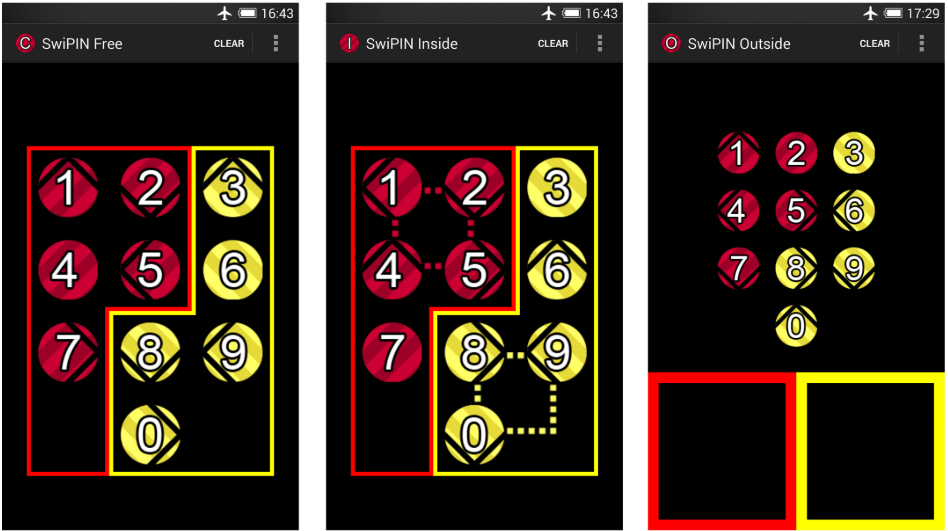
\includegraphics[width=13cm, height=7cm]{Chapters/graphics/swipin.PNG}
\caption{The three variations of \textbf{SwiPIN} by Zezschwitz et al. \cite{Swipin}. The version that was proven to be most usable is \textbf{SwiPIN} \textit{(outside}) on the far right \cite{Swipin}. }
\label{fig:swipin}
\end{figure}


\subsection{Approaches towards Novel Authentication Concepts} \label{2.2.3}
In addition to the earlier discussed research and findings, researchers have also contributed to proposing novel authentication methods. Although their intentions were primarily directed towards solving certain security issues, such as smudge and shoulder surfing attacks (Section \ref{2.1.1}). They also introduced unique authentication methods that have a chance of being more usable than existing ones. Moreover, some made certain discoveries along the way that influence the approach of evaluating usability.\\

Zezschwitz et al. \cite{Swipin} created an interesting mechanism called \textbf{SwiPIN} (see figure \ref{fig:swipin}). It was intended to support the original PIN method in situations in which stronger authentication security is needed. Its main task was to prevent shoulder surfing attacks when users authenticate with their pin. Zezschwitz et al \cite{Swipin} created three variations of the concept, of which one proved to have the best usability of them all, namely \textbf{SwiPIN} \textit{(outside)} (see figure \ref{fig:swipin}). The idea of the concept is to enter the pin through gestures rather than through tapping the buttons (numbers). The interface presents a number pad, and on each of the buttons, there is a black arrow, which indicates the direction in which the gestures should be performed. Also, for each button, a specific color is assigned (yellow or red). To enter one's pin, one would simply perform the gestures of the respective numbers in one of two "boxes" displayed at the bottom of the screen. Gestures of red buttons are performed in the red box and gestures of yellow buttons, in the yellow box (see figure \ref{fig:swipin}). The black arrows, which are assigned to each number, changed for each authentication run. Remarkably, this design increased the effort and memory needed to "successfully" perform a shoulder surfing attack because the attacker must try to memorize the gestures, their order, and the color of the boxes in which they are performed in order to find out which numbers were entered. \\

\begin{figure}[t!]
\centering
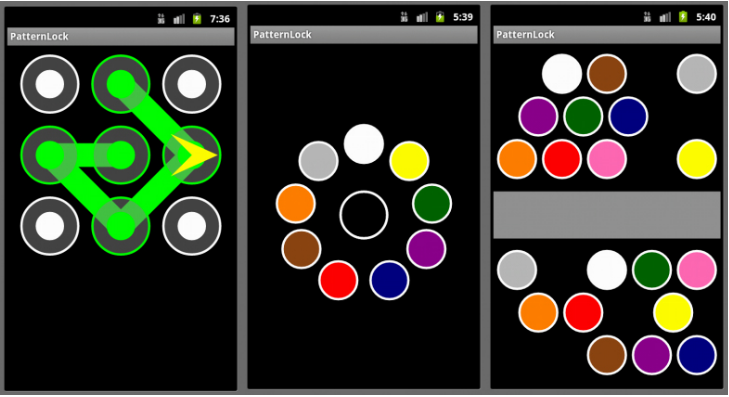
\includegraphics[width=13cm, height=7cm]{Chapters/graphics/graphic.PNG}
\caption{The three concepts made by Zezschwitz et al. \cite{Marbles}. (Left) Pattern 90, a special version of Pattern Rotation, (Middle) Marbles, (Right) Marble Gap, a variation of Marbles.}
\label{fig:marbles}
\end{figure}

Zezschwitz et al. \cite{Swipin} further conducted a study where \textbf{SwiPIN} and the original PIN where compared to each other. They noticed that the utilization of \textbf{SwiPIN} lead to a slightly longer authentication process than PIN. A noticed disadvantage of the concept was that users had to approach it differently than PIN. Since entering a memorized pin into a number pad usually depended on muscle memory, users had to consciously recall their pin, when using \textbf{SwiPIN}. Nonetheless, all participants of the study approved of the concept and imagined themselves using it in risky situations. \\

Another contribution towards designing novel security concepts was made by Zezschwitz et al. \cite{Marbles}. Their goal was to create a protection mechanism against smudge attacks (Section \ref{2.1.1}). They created three concepts: \textbf{Marbles}, \textbf{Marble Gap} and \textbf{Pattern Rotation} (see figure \ref{fig:marbles}). The idea for \textbf{Marbles} was to create an interface that presented colored dots (marbles) aligned in a circular order. The marbles represented the elements that defined a specific password. In order to authenticate, the user would enter their password by dragging the marbles into the center circle in the right order. \textbf{Marble Gap} was based on the same idea, yet differed in its mapping (see figure \ref{fig:marbles}). The marbles were displayed at the top and bottom of the display, separated by a centered rectangle (gap). To enter the password, the user had to drag in the marbles, either from the top or bottom, into the gap. It is important to note that the arrangement and display of the marbles were random for each authentication run in both concepts. The concept of \textbf{Pattern Rotation} was based on the traditional \textit{Android Unlock Pattern} mechanism. The interface presented a 3x3 grid of nodes, which changed its orientation every time a user wanted to authenticate. A special version of \textbf{Pattern Rotation}, Pattern 90, enabled four different grid orientation (see figure \ref{fig:marbles}). \\

To examine which one of the three concepts users' preferred best in terms of usability and effectiveness, Zezschwitz et al. \cite{Marbles} conducted a study in which all three concepts were analyzed. They adopted an interesting approach to measure the authentication times by dissecting the authentication process into "orientation" and "input" time. Interestingly, Harbach et al. \cite{AnatomySmartphone} made a similar approach when they analyzed the difference between PIN and PATTERN (Section \ref{2.2.2}). Zezschwitz et al. \cite{Marbles} defined the "orientation" time as the period between the beginning of the authentication and the first input event of the user. Also, they interpreted the input time as the period between the first input event and the moment in which the input is either approved or canceled. Through this distinction, they realized that the factor of randomization in each of the concepts affected their overall authentication time in different ways. For instance, in \textbf{Marbles} and in \textbf{Marble Gap}, randomization was shown to elongate the "input" time, because the marbles, which had to be searched for during the input, were positioned differently every time. In contrast, the orientation time of \textbf{Pattern Rotation} was increased through randomization because participants needed more time to familiarize themselves with the current position of the grid. Another discovery made, through the distinction of "orientation" and "input", was participants' perception of speed. While \textbf{Pattern Rotation} was measured to be the second quickest of all three, participants rated it as the slowest. However, \textbf{Pattern Rotation} did have the longest "orientation" time. This discovery allowed Zezschwitz et al. \cite{Marbles} to realize that users disliked mechanisms that had a long "orientation" time. Therefore, \textbf{Pattern Rotation} was considered not usable. Security analysis also showed it was not sufficiently secure. In contrast, participants approved of \textbf{Marbles} and \textbf{Marbles Gap} and considered them very usable.\\


Looking back at the research contributions discussed in this section, we notice that one of the main reasons why users were found to consciously discard authentication mechanism was due to "inconvenience" \cite{Albayram:2017:BUL:3235924.3235929, Harbach:2016, Alsaleh}. Despite attempting to attract smartphone users to use screen locks by informing them about their effectiveness and purpose \cite{Albayram:2017:BUL:3235924.3235929}, a decent amount of study participants were found to have not improved their security behavior. As mentioned earlier, smartphone users were claimed to agree on using a screen lock, if the particular mechanism promised to be faster than the already existing ones \cite{AnatomySmartphone}. This indicates that users prefer efficiency over effectiveness. However, previously discussed findings by Zezschwitz et al. \cite{PatternWild} have shown that the efficiency of an authentication mechanism can not be determined by the time that it requires for unlocking. For instance, although PIN proved to take less time to authenticate than PATTERN, study participants preferred the PATTERN mechanism better \cite{PatternWild}. Reason being, that with PIN, users had to prepare longer for authentication than with PATTERN \cite{AnatomySmartphone}. Consequently, we learned that in order to examine the efficiency of a particular authentication mechanism, we can not solely rely on comparing their measured input time. This revelation was backed by the approach of Zezschwitz et al. \cite{Marbles}. By dividing the overall authentication process distinctively into "orientation" and "input" time, they not only understood users' perception of efficiency better but were also able to detect how differently certain design choices (e.g., randomization) could influence the anatomy of particular authentication mechanisms. \\

Thus users' were discovered to perceive interactions that require less cognitive effort to be more efficient and faster. We have learned that the measured efficiency of authentication mechanisms can not be set equivalent to their perceived efficiency \cite{anonymous}. On that note, examining the factors that affect perceived efficiency could be a productive step towards better understanding what types of mechanism designs users approve of, or discard. In that way, researchers could evaluate existing and newly designed authentication mechanisms, and also compare them to each other, in the same manner. This introduces the primary goal of our thesis, which is to contribute towards finding a standard through which we could generalize an evaluation method for usability, with a focus on perceived efficiency. In the course of this thesis, we will base our work on the findings made in an unpublished paper by Anonymous et al. \cite{anonymous}. In their paper, they grasped the notion of dissecting authentication time and proposed a novel method of rating usability according to users' perception, rather than quantitative measurements. To provide a basic comprehension of our work throughout this thesis, we will introduce and explain their remarkable approach in Chapter \ref{ch:third}. 







%\addtocontents{toc}{\protect\clearpage} % <--- just debug stuff, ignore

%*****************************************
\chapter{Theoretical Foundation and Hypotheses}\label{ch:third}
%*****************************************

In the following chapter, we will present an unpublished scientific work that will serve as the theoretical core of our thesis. This scientific paper goes by the title 
\begin{center}
 \textit{"Designing Efficient Authentication Mechanisms: There is More to Efficiency than Input Speed."}   
\end{center}
Thus the authors remain unknown. We will refer to them as Anonymous et al. \cite{anonymous} in the following course of this thesis. As implied in Section \ref{2.2}, our intention for this chapter is to introduce an interesting contribution made towards setting a standard for the evaluation of efficiency in smartphone authentication mechanisms. We will begin by presenting the findings of Anonymous et al. \cite{anonymous}. Then, we will proceed by elaborating on the limitations of their approach. Lastly, we will explain how we intend to validate their findings by reevaluating their approach and proving their hypotheses.

\section{Approach}

As discussed in Chapter \ref{ch:second}, the lack of usability in various authentication mechanisms, has been the main reason why many smartphone users refuse to use a screen lock for their phones. In Section \ref{2.2}, we saw how researchers attempted to make authentication mechanisms more usable by increasing their perceived effectiveness. Unfortunately, this approach was only successful to a certain extent and was not sufficiently productive for solving the usability issue. We learned that users generally value efficiency over effectiveness when it comes to authentication mechanisms and would prefer no screen lock rather than using one that is time-consuming and inconvenient (see Section \ref{2.2}). Consequently, researchers tried to detect the factors that most affected the efficiency of smartphone security and realized that these factors could not be assessed by simply measuring the duration of the input. They noticed a factor that had often been disregarded during the evaluation of efficiency, and that is \textit{mental effort} (see Section \ref{2.2}). The amount of mental effort that is needed to accomplish an authentication task is crucial for user-acceptance \cite{anonymous}. Therefore, new measurement methods are in need which approach the practice of authentication on a human level and are designed with respect to humans' perception of time and cognitive abilities. \\


To that, Anonymous et al. \cite{anonymous} made an effort to create a measurement standard for evaluating the usability of authentication mechanisms in terms of their efficiency \cite{anonymous}. They noticed how previous studies indicated that users commonly prefer authentication mechanisms that require little to no mental effort \cite{anonymous, AnatomySmartphone}. Moreover, they realized that those mechanisms were the ones to be rated most usable and fastest to use. Researchers made these revelations possible, by categorizing the overall authentication time into \textbf{orientation} and \textbf{input} times \cite{anonymous}. Anonymous et al. \cite{anonymous} also analyzed the danger that occurred from only considering input times in evaluations. Thus it can lead to false conclusions about the efficiency of authentication mechanisms. This is specially the case when mechanisms are set in comparison to each other \cite{anonymous}. \\

\begin{figure}[t!]
\centering
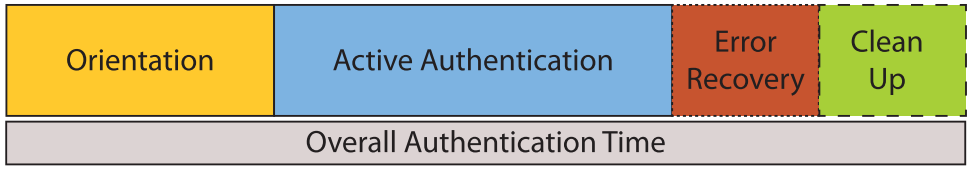
\includegraphics[width=15cm, height=3cm]{Chapters/graphics/Phases.PNG}
\caption{Component phases of an authentication process. While Orientation and Active Authentication (input) phase are the core components of an authentication procedure, Error Recovery may also be included. Clean up phases are not considered part of the authentication process, yet in some designs they are crucial for its completeness \cite{anonymous}. }
\label{fig:phases}
\end{figure}

Anonymous et al. \cite{anonymous} began by reinterpreting the architecture of the general smartphone authentication process (see figure \ref{fig:phases}). Next, they subdivided the overall authentication period into the following phases \cite{anonymous}: 

\begin{itemize}
    \item \textbf{\textcolor{orange}{Orientation:}} In previous research, this phase was commonly defined as the \textit{preparation} phase \cite{anonymous}. It defines the period, beginning from the moment a smartphone screen is switched on, to the moment when the first input action is made \cite{anonymous}. It usually takes place before the user enters their secret. This is the time which they spend either recalling their secret, preparing themselves for its input, or both \cite{anonymous}. It is considered to be the part of the authentication process which requires the most mental effort \cite{anonymous}.  
    \item \textbf{\textcolor{blue}{Active Authentication:}} This phase defines the time a user needs to enter their secret. It begins with the very first input action and ends with the very last\footnote{By \textit{last input action}, we mean the moment which determines whether unlocking is permitted or denied \cite{anonymous}.}. We will call this phase the \textbf{input} phase, for simplicity reasons.
    \item \textbf{\textcolor{red}{Error Recovery:}} This phase is useful in situations where the user makes an input error. Its purpose is to signify the user that an error has occurred and to provide the possibility of recovering from it by making the user restart the authentication process, or by allowing so called \textit{undo operations}, which allow the user to correct their mistake and proceed with the input. 
    \item \textbf{\textcolor{green}{Clean Up:}} This phase is not considered to be a solid part of the authentication process, yet in some newly developed mechanisms, it is crucial for completing the authentication. An example for its use, is found in the concepts \textbf{TinyLock} by Kwon et al. \cite{kwon} and \textbf{Whispercore} by Airowaily et al. \cite{Airowaily}. In these designs, the clean up phase is intended to remove oily residues on the smartphone screen and thereby counteract the chance of potential smudge attacks \cite{anonymous}. 
\end{itemize}

The two phases which are considered to be highly essential for the authentication process are the \textit{orientation} and \textit{input} phases. In previous approaches, the \textit{input} phase has often been considered to define the actual authentication procedure. Consequently, \textit{orientation} time was often disregarded and ignored in usability evaluations. \textit{Error recovery} is a phase that is not essentially mandatory for authentication, yet very useful for error management. Anonymous et al. \cite{anonymous} find that its implementation can have a significant effect on the efficiency of an authentication mechanism. In some cases, its implementation can cause for further \textit{orientation} or \textit{clean up} phases \cite{anonymous}. This, in return, may cause a longer authentication duration. The implementation of the \textit{clean up} phase depends on the design of the authentication concept. Authentication is possible with or without it. \\

By outlining the structure of the authentication process, Anonymous et al. \cite{anonymous} made a collection of observations and factors which they wanted to regard and prove in a user case study. First, they wanted to consider how authentication phases are proportioned. Reason being that it has a significant influence on the perceived efficiency of mechanisms. Moreover, the longer the \textit{orientation} time of an authentication mechanism is, the slower and less efficient it is perceived. In fact, cases in which the duration of the \textit{orientation} phase exceeds the \textit{input} phase, have been seen to be widely disliked by users. \\

Second, they wanted to consider how authentication phases are ordered in an authentication process \cite{anonymous}. Thus this factor may highly differ amongst authentication concepts, such as Pattern Rotation and Marbles \cite{Marbles} (Section \ref{2.2.3}), it is very important to regard. For instance, Pattern Rotation only consists of two phases, with the \textit{orientation} phase preceding the \textit{input} phase. Marbles, on the other hand, has multiple small \textit{orientation} and \textit{input} phases, ordered in an alternating manner. Interestingly, Anonymous et al. \cite{anonymous} find that the latter has the possibility of decreasing the perceived duration of authentication. \\

Third, they want to regard the coherence of \textit{orientation} and \textit{input} phases in terms of their contexts. Thus it also has a significant impact on a mechanism's perceived efficiency \cite{anonymous}. Meaning, the less coherent the contexts of \textit{orientation} time and \textit{input} time are, the less efficient and convenient they are perceived. This factor was regarded in the design of Marbles \cite{Marbles}. Thus its tasks alternate between finding the marbles and entering them, the contexts of the tasks complement each other. Through further research Anonymous et al. \cite{anonymous} found that humans tend to perceive periods longer than they are if the contexts of these periods are incoherent \cite{anonymous,perception}.\\

Lastly, Anonymous et al. \cite{anonymous} state that \textit{error recovery} should be cautiously managed throughout the authentication of a mechanism \cite{anonymous}. As mentioned above, the implementation of \textit{error recovery} may result in further \textit{orientation} and \textit{clean up} phases. This observation was shown in findings by Zezschwitz et al. \cite{PatternWild}, discussed in section \ref{2.2}. They discovered how users tended more towards Pattern authentication than Pin because it managed errors better. Even though Pattern took longer to authenticate with than Pin. This is because Pin allowed to manage errors through \textit{undo-operations}. These have shown to be disliked and therefore are seldom used in designs \cite{PatternWild, anonymous}. 

\begin{figure}[t!]
\centering
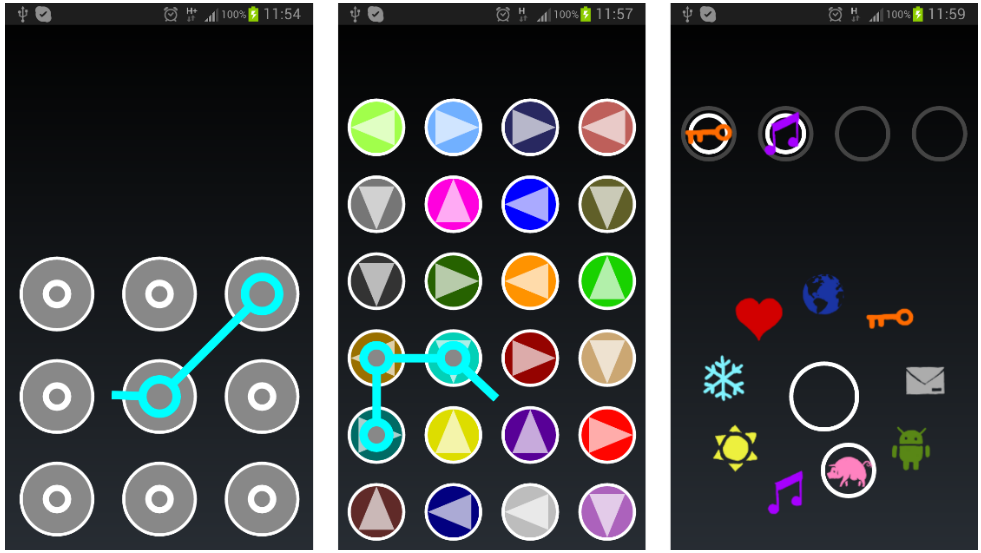
\includegraphics[width=14cm, height=7cm]{Chapters/graphics/androidPatternMarble.PNG}
\caption{The concepts that Anonymous et al. \cite{anonymous} used in their study. Left: Android Unlock Pattern (baseline); Middle: Pattern Rotation; Right: Marbles. See figure \ref{fig:marbles} to see how the concepts were modified \cite{anonymous}.}
\label{fig:android}
\end{figure}

\section{User Case Study}

To prove their assumptions and observations, Anonymous et al. \cite{anonymous} decided to focus mainly on the phases, \textit{orientation}, and \textit{input}. Thus they are the most important phases during authentication. They selected three authentication concepts, each representing a different ratio of \textit{orientation} and \textit{input} time \cite{anonymous}
\footnote{To better understand the functionalities of the concepts listed above, we recommend revisiting the approach by Zezschwitz et al. \cite{Marbles}, presented in Section \ref{2.2.3}.}: 

\begin{itemize}
    \item \textbf{Android Unlock Pattern} presented a \textcolor{red}{short} orientation - \textcolor{red}{short} input ratio,
    \item \textbf{Pattern Rotation} presented a \textcolor{blue}{long} orientation - \textcolor{red}{short} input ratio,
    \item \textbf{Marbles} presented a ratio in which orientation and input time were interlaced.
\end{itemize}

It is important to note that \textit{Pattern Rotation} and \textit{Marbles} \cite{Marbles} were slightly modified in this study. \textit{Pattern Rotation} presented a larger grid than the original design, and in \textit{Marbles}, the elements (marbles) were small images rather than colors only (see figure \ref{fig:android} and \ref{fig:marbles}. All three concepts were implemented in a prototype which was intended to be installed on the Android smartphones of study participants \cite{anonymous}. The prototype was intended to serve as an authentication system on the participants' phones. Each of the concepts was planned to be tested for ten days \cite{anonymous}. After each ten-day period, an online survey was required to be taken. Also, during the concept-tests, \textit{orientation} and \textit{input} times were logged for each authentication \cite{anonymous}. \textit{Orientation} time was logged from the moment the screen was switched on, to the first input event. \textit{Input} time was logged from the first to the last input event \cite{anonymous}. Participants were allowed to choose their secrets for the concepts. However, patterns for \textit{Android Unlock Pattern} had to consist of six nodes, patterns for \textit{Pattern Rotation} had to have five nodes, and secrets in \textit{Marbles} had to consist of four elements \cite{anonymous}.

\subsection{Results}

The study yielded 19 participants and delivered a set of 18 valid data entities \cite{anonymous}. Anonymous et al. \cite{anonymous} wanted to examine the different outcomes that result when authentication times are analyzed differently. First, they analyzed the overall authentication times of the concepts and noted the following ranking in regarding the \textbf{measured performances}\footnote{The concepts are ordered from fastest to slowest (or best to worst) in this and the following rankings of this section.} \cite{anonymous}:

\begin{enumerate}
    \item \textbf{Android Unlock Pattern},
    \item \textbf{Pattern Rotation},
    \item \textbf{Marbles}.
\end{enumerate} 

However, when they analyzed the \textit{input} times of each other concepts only, they noticed the following difference:

\begin{enumerate}
    \item \textbf{Pattern Rotation},
    \item \textbf{Android Unlock Pattern},
    \item \textbf{Marbles}.
\end{enumerate}

Last, they analyzed the \textit{orientation} time of the concepts and realized another significantly different outcome. \textit{Android Pattern Unlock} required the least amount of mental effort and therefore had the shortest \textit{orientation} time, on average \cite{anonymous}. Interestingly, there was hardly any difference between \textit{Pattern Rotation} and \textit{Marbles}, in terms of their average \textit{orientation} times \cite{anonymous}. The \textbf{perceived efficiency} of the concepts was rated qualitatively through five-point Likert scales \cite{anonymous}. Results showed that \textit{Android Unlock Pattern} was seen as the fastest of all three concepts. More than half of the participants considered \textit{Marbles} to be efficient, despite it being measured slower than \textit{Pattern Rotation}. Moreover, half of the participants perceived \textit{Pattern Rotation} as efficient \cite{anonymous}. Also, participants ranked the concepts in the following when asked if they contented a fast and easy orientation \cite{anonymous}: 

\begin{enumerate}
     \item \textbf{Android Unlock Pattern},
    \item \textbf{Marbles},
    \item \textbf{Pattern Rotation}.
\end{enumerate}

Lastly, when asked about the required cognitive effort, all participants approved of Android Pattern Unlock requiring the least amount of mental effort, followed by Pattern Rotation, then Marbles \cite{anonymous}. \\

STILL HAVE TO ANALYZE THE RESULTS

\section{Limitations and suggestive improvements}

In this section, we will first begin by reporting some limitations of the study, given by Anonymous et al. \cite{anonymous}. Then we will proceed by sharing our observations on specific qualities of the study, which we attempt to modify and improve to make their findings and observations universally valid.  

First, Anonymous et al. \cite{anonymous} state that the overall perception of the tested concepts could have been influenced by the participants' general preference \cite{anonymous} because a person's culture and history have shown to influence their acceptance of a particular system \cite{Harbach:2016} (Section \ref{2.2.1}). We intend to exclude this limitation by developing a prototype in which the particular ratios are represented through the same concept. That way, we will, hopefully, receive more a genuine evaluation of the ratios, without any interference of participants' preferences regarding a particular concept. Moreover, Anonymous et al. \cite{anonymous} state that the measured times for \textit{orientation} might differ from the actual times \cite{anonymous}. Reason being that the measurements for the \textit{orientation} times began as soon as the smartphone screen was turned on, and it is not guaranteed that authentication was the only immediate action after this event \cite{anonymous}. We plan on rectifying this possible inaccuracy, by isolating the \textit{orientation} phase from any other possible action. We will design our concept in a way that requires the user to initiate the authentication process actively, such that we can define a fix starting point for the \textit{orientation} time for the measurement.\\

Furthermore, we observed that the chosen ratios by Anonymous et al. \cite{anonymous} might not have been suitable enough to receive a definite result on whether users truly prefer short \textit{orientation} over long \textit{orientation}. We think it would be interesting to observe the outcome of testing ratios that have the same temporal arrangement, yet are contrasting regarding the lengths of their phases. Thus not included by Anonymous et al., we consider including the ratio \textit{short orientation - long input} into our analysis. We imagine that by mainly focusing on the ratios \textit{long orientation - short input} and \textit{short orientation - long input}, and by setting the ratio \textit{short orientation - short input} ratio as a baseline, we could receive more detailed results on users' attitude towards authentication concepts with different lengths of \textit{orientation} phases. Also, we could observe how far different lengths of \textit{input} phases might play a role in their preference and perception of efficiency. Lastly, we suggest that by letting participants qualitatively evaluate the ratios in comparison to each other, we hope to receive more detailed and precise information about their preferences.  





%*****************************************
\chapter{Developing an Interaction System}\label{ch:forth}
%*****************************************


Before entering into the design process it is crucial to mention that the following interaction system was created solely to serve as a tool in the user case study, which will be presented in Chapter 5. The use of this system was not intended for any use outside of the contributions for this thesis. Therefore certain aspects such as security and effectiveness have not been considered during the design and the development of this system. Nonetheless, during its creation, we tried our best to follow the steps of a User-Centered Design (UCD) approach and included a selection of Human Computer Interaction (HCI) principles, in order to make the system easier on the human eyes and on the mind. It was important to make sure that the design and structure choices, neither distracted the user from the important factors of the study, nor complicated the effort needed to concentrate on them.  

\section{Requirements of the design for the study}
As mentioned above, the interaction system was intended to be utilized to help examine certain factors later on in the study. These factors were \textbf{orientation time} and \textbf{input time}, previously explained in Chapter 3. In order to do so, the interaction system had to be based on a certain concept. This concept had to be divided into two coherent and related miniature tasks: a mental task and a practical task. The intention behind this division is to measure the overall time needed for the accomplishment, thereby distinguishing between the duration of the mental task (orientation time) and the duration of the practical task (input time). \\

In order to validate the findings presented in the previous chapter, we had to find a way through which we could examine the effect of orientation time on authentication, with respect of the input time. Therefore we decided to analyse two contrasting time ratios: 
\begin{center}
    \textbf{Long} orientation - \textbf{Short} input \\
    vs. \\
    \textbf{Short} orientation - \textbf{Long} input
\end{center} 

In contrast to the study by Anonymous et al. \cite{anonymous}, we wanted to directly examine the influence that orientation time has on users' acceptance of an authentication concept, by comparing both contrasting variations against each other, using only one concept, instead of three. Therefore the concept had to be malleable in a way, such that the time needed to accomplish the miniature tasks, could be modified by adjusting their degree of difficulty and complexity. We imagined the less difficult and the less complex the task, the less time is needed for its accomplishment, and vice versa. This approach applied the mental task, as well as the practical task. 

Another crucial requirement of the design, was that it included a built-in timer, that would measure the duration of the tasks separately and thereby deliver us the orientation and input needed.  

\section{Concept Development}








%*****************************************
\chapter{Case Study}\label{ch:fifth}
%*****************************************

The following chapter presents a user case study which was intended to complement and validate the findings made by Anonymous et al. \cite{anonymous} (see Chapter \ref{ch:third}). The chapter begins by introducing the design of the user case study. Next, the demographic of the recruited participants is presented, followed by a documentation of the study's procedure. Last, the quantitative and qualitative results of the study are discussed. The goal of the research contribution was to examine the effect of \textit{orientation time} on the perceived efficiency of authentication mechanisms. 

\section{Design} \label{5.1}

The user case study was designed as a field study which was conducted in two destinations: on campus of the computer science department at Rheinische Friedrich-Wilhelms-Universit{\"a}t Bonn (Uni Bonn) and at the author's home residence. The independent variable was \textit{ratio} and it had three levels:
\begin{enumerate}
    \item \textcolor{blue}{long} orientation/\textcolor{red}{short} input (abbrv. \textit{long/short}), 
    \item \textcolor{red}{short} orientation/\textcolor{blue}{long} input (abbrv. \textit{short/long}), 
    \item \textcolor{red}{short} orientation/\textcolor{red}{short} input (abbrv. \textit{short/short}). 
\end{enumerate}

The implemented concept \underline{\textbf{FiPa}}, presented in Chapter \ref{ch:forth}, served as a medium to represent the ratios of interest. The order of the ratios was counterbalanced amongst the participants (see figure \ref{fig:permutation}). Data was collected quantitatively by measuring the \textit{orientation} and \textit{input time} for each of the ratios, as explained in Chapter \ref{ch:forth}. Data was also collected qualitatively through a questionnaire, which required study participants to evaluate the aesthetic of the application\footnote{Although this is slightly beyond the scope of the research, I was interested in seeing whether the design of the application had an impact on participants' performance. These observations will be presented later in Chapter \ref{ch:sixth}.}, the ratios (\textit{long/short} and \textit{short/long}), and to also choose which of the two ratios they preferred most. On average, the duration of the study was 20 minutes per participant. 

\section{Participants} \label{5.2}

Twenty-five participants were recruited for the study. Initially, students were informed about the study through a social platform for computer science students at Uni Bonn. Another part was collected on campus of the university's computer science department, and four participants were acquaintances of the author of this thesis. There was no premise for participating in the study, meaning anyone was eligible to partake. Participants who made input-errors (see Section \ref{4.3.2}) were excluded from the evaluation. Nineteen valid data entities remained, of which 13 (62.4\%) were male and 6 (31.6\%) were female. The average age was 21 years, with 17 being the youngest and 31 being the oldest age. The majority of the participants (78.9\%) had an IT-Background and were computer science students. Also, all participants, except for one, used a screen lock for their smartphones: 42.1\% used \textit{Pin}, 36.8\% used \textit{Pattern}, and 15.8\% used \textit{Password} (see figure \ref{fig:demo}). 

\begin{figure}[t!]
\centering
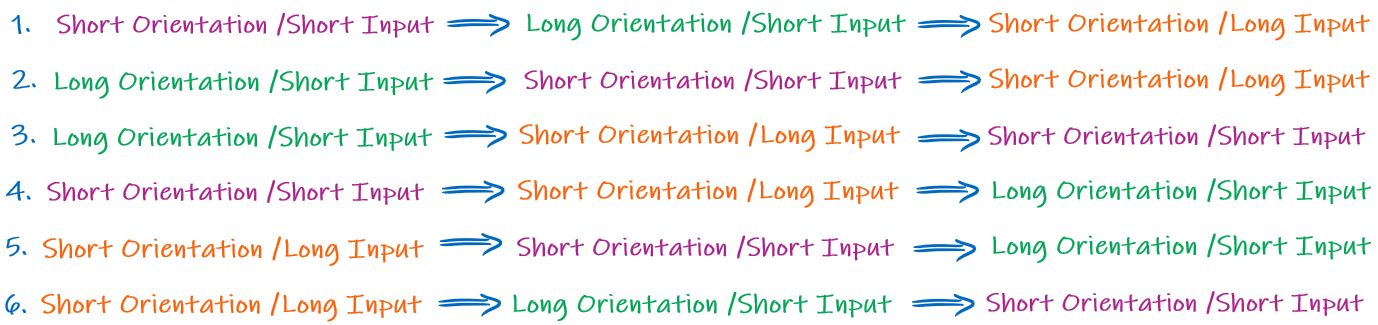
\includegraphics[width=14cm, height=4cm]{Chapters/graphics/permutation.PNG}
\caption{The order in which the three ratios were counterbalanced amongst the participants during the study.}
\label{fig:permutation}
\end{figure}


\section{Procedure} \label{5.3}
The study was held for each participant, separately. First, the experimenter provided a introduction on the study purpose to the participant:

\begin{center}
\textit{Analysis of certain factors of a smartphone authentication process that might play a role in its perceived efficiency.}    
\end{center}

It was also emphasized that the improvement of usability in authentication mechanisms was of interest and that the security aspect was outside the scope of this research study. Moreover, participants were assured that the testing of \underline{\textbf{FiPa}} was not intended to evaluate their cognitive skills or intelligence. It also was important that they felt comfortable and that they did not feel nervous or put under pressure during the course of the study, as it could impact negatively validity of the obtained results.\\

Next, the experimenter described the structure of the application, representing the concept \underline{\textbf{FiPa}}. They explained to the participant that it was meant to emulate an activity, which resembled an authentication concept. They explained the application presented a series of small "challenges", for the participant to solve\footnote{"Challenges"  meant the \textbf{mental} and \textbf{practical tasks}, explained in Chapter \ref{ch:forth}.}. The simple challenges were demonstrated with the help of the paper prototype, shown in figure \ref{fig:paperprototype}.\\

\begin{figure}[t!]
\centering
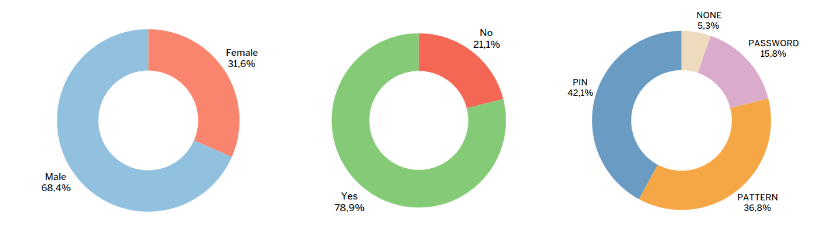
\includegraphics[width=15cm, height=5cm]{Chapters/graphics/Demos.PNG}
\caption{Demographic information on the \textit{gender} (Left), \textit{IT-Background} (Middle), and the \textit{personal screen lock choice} (right) of the recruited participants.}
\label{fig:demo}
\end{figure}

After ensuring that the participant had no further questions, the experimenter proceeded by presenting the application to the participant. The application was installed on an Android smartphone provided by research group of Dr. Emanuel von Zezschwitz.\\
First, the participants were advised to begin with the training-segment of the application, presented in section \ref{4.3.2} (see figure \ref{fig:flow}). The purpose of the training-segment was to ensure that the participant understood the concept of \underline{\textbf{FiPa}} and to reduce the number of errors in the quantitative data set. As mentioned in Section \ref{4.3.2}, the participant was allowed to repeat the training-segment, until they felt ready to start with the actual testing the concept. During the training-segment, the experimenter guided them through the process, when help was needed, and explained certain features, such as the \textit{error-recovery} and the method of input. \\

When the participant felt ready to start the test, the experimenter entered a unique \textit{user-id} for the participant. The experimenter did not intervene, as the participant was executing the actual test of the application. Once the participant was done, they were given a questionnaire to fill out (see Appendix \ref{ch:appendix}). At the end of the study, each participant was compensated with 5 Euros.

\section{Results} \label{5.4}

\begin{figure}[t!]
\centering
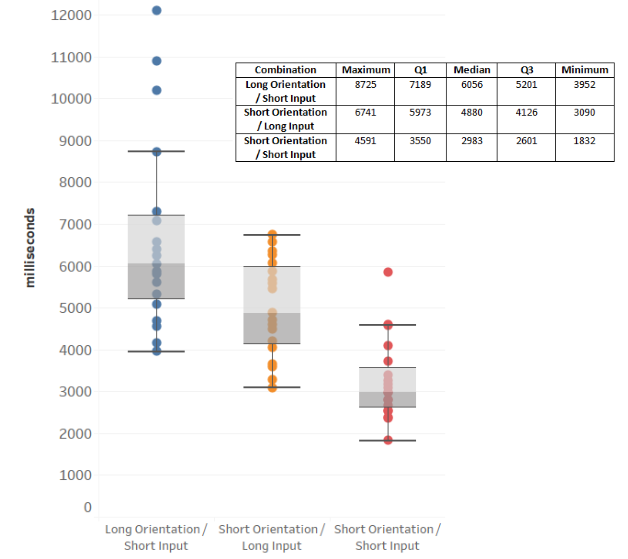
\includegraphics[width=13cm, height=11cm]{Chapters/graphics/Combinations.png}
\caption{A plotted representation of the overall times for each ratio, presented in the study.}
\label{fig:combination}
\end{figure}

\subsection{Measurements}

 As mentioned earlier, \textit{orientation} and \textit{input times} were measured for each ratio. , each \textit{combination} presents three different challenges (couples, see Section \ref{4.2.2.4}). Analogous to the measurement approach, presented in section \ref{4.2.2.4}, the first and second challenge of each combination were considered to be an exercise for the user. Despite the training-segment, participants made a significant amount of mistakes during the first two levels of each phases, and made very little to non in the third. After excluding all data entities which contained unsuccessful input activities, 19 clean data sets remained. \\

Although, the ratios \textit{short/long} and \textit{long/short} (see Section \ref{5.1}) were designed to have the same overall length/duration, results show that they had a temporal difference of 1176 ms, on average (see figure \ref{fig:combination}). The combination \textit{long/short} (6056 ms) had the longest duration, followed by \textit{short/long} (4880 ms) and, lastly, \textit{short/short} (2983 ms) (see figure \ref{fig:combination}). Figure \ref{fig:times} shows that, on average, participants needed notably more time (1094 ms) to finish the long \textit{orientation phase} of \textit{long/short} than they needed for the long \textit{input phase} of \textit{short/long}. If we observe the maximum values of both ratios (see Figure \ref{fig:times}), we notice that one participant needed a maximum time of 9053 ms for long \textit{orientation}. However, the remaining participants' time long \textit{orientation} did not exceed 5202 ms. This implies that for the majority of the time, long \textit{orientation} and long \textit{input} did not significantly differ from each other regarding their measured times. \\
In contrast, the ratios \textit{long/short} and \textit{short/long} differed less notably in terms of the short phases, namely short \textit{orientation} and short \textit{input}. On average, they differed in 572 ms. Nonetheless, participants needed more time for the short \textit{orientation phase} than they needed for the short \textit{input phase} (see figure \ref{fig:times}).

As mentioned earlier in Section \ref{4.1}, the ratio \textit{short/short} was meant to serve as a baseline to the time measurements. By comparing the duration of the phases which \textit{long/short} and \textit{short/long} share with the baseline ratio, it is noticeable that their short \textit{orientation phases} have a difference of 261 ms, whereas the short \textit{input phases} only differ in 2 ms (see figure \ref{fig:times}).  

\begin{figure}[t!]
\centering
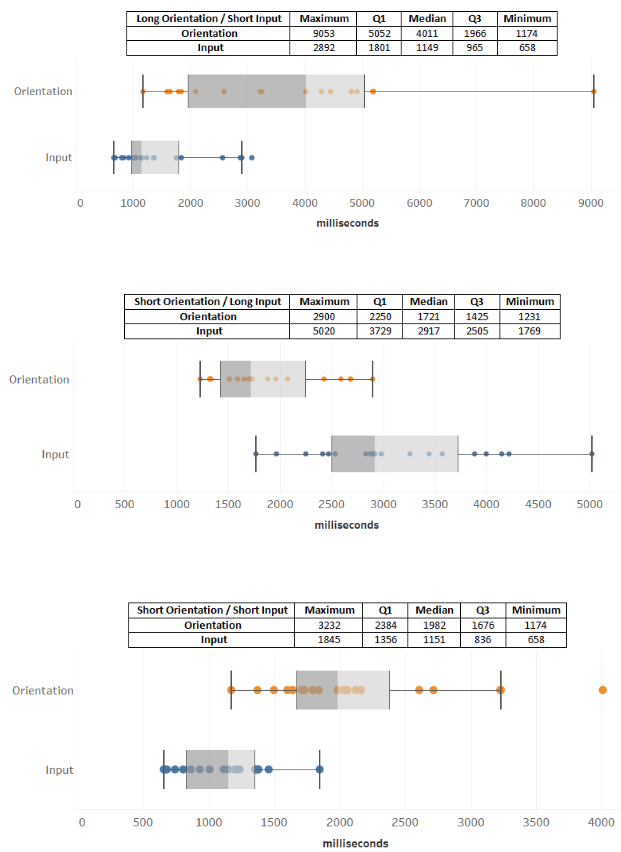
\includegraphics[width=14cm, height=20cm]{Chapters/graphics/Times.png}
\caption{A plotted representation of the time measurements for each ratio, presented in the study: \textit{long/short} (Top);  \textit{short/long} (Middle); \textit{short/short} (Bottom).}
\label{fig:times}
\end{figure}

\subsection{Users' Perception}

A qualitative evaluation of the ratios \textit{long/short} and \textit{short/long} was assessed through a questionnaire (see Appendix \ref{ch:appendix}). As proposed in Section \ref{3.3}, in the questionnaire, the ratios \textit{short/long} and \textit{long/short} were compared to each other, to obtain a precise insight on which of both participants generally preferred more. To ensure the participants had a clear conception of the mentioned ratios, they were given an illustration as an aid to refer to, as they filled out the questionnaire (see figure \ref{fig:illustration}). First, participants were asked to evaluate both ratios separately, through five-point Likert scales (see figure \ref{fig:survey2}, questions 11-12). \\

When participants were asked whether they found the searching process (\textbf{mental task}) of ratio \textit{long/short} annoying, the answers were split between \textit{agree} (8) and \textit{disagree} (8). Three participants found no difference between the two combinations (see figure \ref{fig:likert}). Most participants were able to memorize (89\%) and enter (84\%) the pattern (\textbf{practical task}) easily (see figure \ref{fig:likert}). \\
In contrast, all participants disagreed that the search process \textit{short/long} was annoying. Moreover, all agreed that the pattern was easy to memorize and 89\% agreed that it was easy to enter (see figure \ref{fig:likert}).\\
 
 \begin{figure}[t!]
\centering
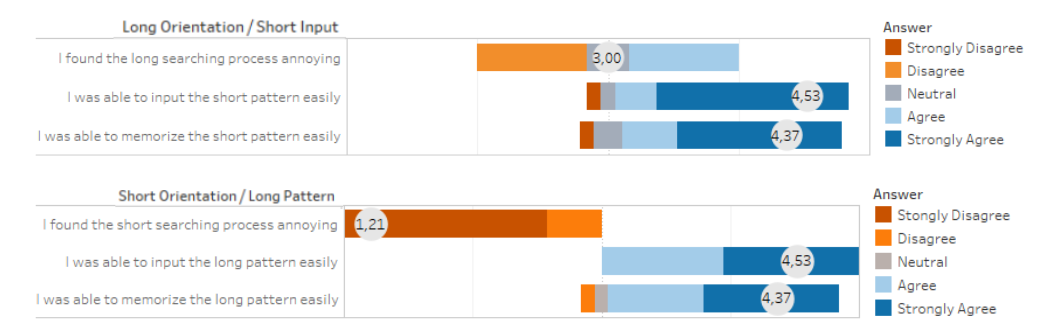
\includegraphics[width=15cm, height=5cm]{Chapters/graphics/Likert1213.PNG}
\caption{A representation of how participants evaluated each ratio separately in terms of this mental and practical task: \textit{long/short} (Top); \textit{short/long} (Bottom).  }
\label{fig:likert}
\end{figure}

Next, participants were asked certain actively choose which ratio they preferred best in terms of certain given characteristics (see figure \ref{fig:likert2}). This evaluation of the ratios was also assessed through Likert scales (see figures \ref{fig:survey2}, \ref{fig:survey3}, questions 13-19). The majority of the participants (68\%) found that \textit{long/short} required more mental effort, about 16\% chose \textit{short/long} and another 16\% saw no difference between both ratios (see figure \ref{fig:likert2}). \\
Moreover, about 79\% voted for \textit{short/long} as the easiest, followed by a 16\% finding \textit{long/short} easier, followed by 5\% who saw no difference between the two (see figure \ref{fig:likert2}). Participants were also asked to chose the ratio, which they found was took longer to find. All participants agreed that the pattern for \textit{long/short} took longer to find (see figure \ref{fig:likert2}). In contrast, participants were asked which pattern they found took longer to enter. Seventy-four percent chose \textit{short/long}, 26\% saw no difference, and 0\% chose \textit{long/short}. Lastly, participants were asked which combination they found was more efficient. The majority 58\% found that \textit{short/long} was more efficient, followed by 26\% chose \textit{long/short}, and 16\% who saw no difference (see figure \ref{fig:likert2}). \\

If we compare the participants' estimation, regarding which ratio had the longest duration, to the actual time measurements, we will find that 36\% (4) misestimated and thought \textit{long/short}, whereas \textit{short/long} was true. Nonetheless the majority of the participants (64\%) estimated correctly. In addition, 18\% percent (2) thought that \textit{short/long} took longer to enter and 36\% (4) didn't perceive a difference, whereas \textit{long/short} was actually true for both cases. Regarding the estimations of the overall duration of the ratios, five participants (26\%) misestimated. In four cases, \textit{long/short} was considered longer, although \textit{short/long} was true. The remaining case found that \textit{long/short}, although the opposite was true. In addition, two participants saw no difference between both combinations, while \textit{short/long}  actually took longer time, for both. \\

\begin{figure}[t!]
\centering
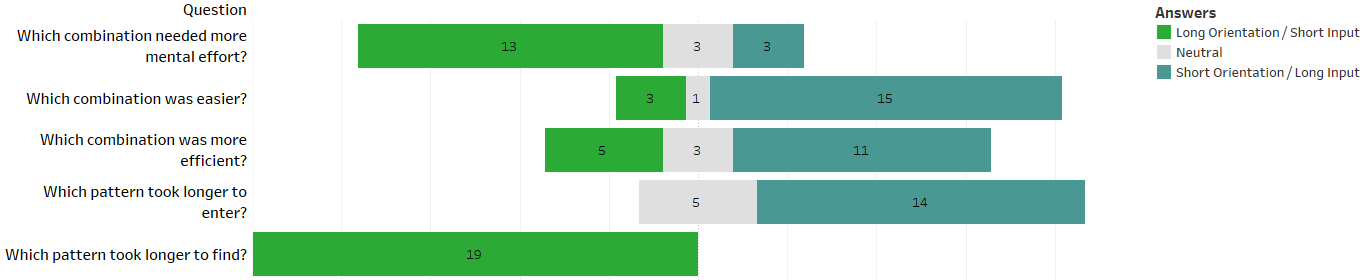
\includegraphics[width=15cm, height=4cm]{Chapters/graphics/Likert2.png}
\caption{Participants were asked to compare the combinations \textit{long/short} and \textit{short/long} to each other by answering the questions above. These questions were answered using Likert scales. }
\label{fig:likert2}
\end{figure}

To get a clearer understanding of the participants' preferences, they were asked to declare which ratio they would prefer for the screen of their smartphone. They were advised to elaborate on their choice based on four given reasons to choose from (see figure \ref{fig:survey3}, question 20): \textit{It's more efficient / more secure / more difficult / challenging}\footnote{Multiple answers were possible.}.\\
Forty-two percent (8) preferred \textit{long/short}, whereas 47\% (9) preferred \textit{short/long} (see figure \ref{fig:preference}). Most frequent reasons given for choosing \textit{long/short} were that is was \textit{more secure} and \textit{more difficult}. Only one participant found that it \textit{more efficient} and only two found that it was \textit{challenging}. Interestingly, one participant elaborated further on their choice and wrote that \textit{short/long} also was more comfortable to use.\\

In contrast, 47\% favored the ratio \textit{short/long} and most frequent reasons given were \textit{more secure} and \textit{more efficient}. The reasons \textit{more difficult} and \textit{challenging} were only given once, each. Two participants elaborated that they would choose \textit{short/long} because it is easier, for when they are tired. Eleven percent (2) chose neither of both ratios and elaborated on their choice in the following (see figure \ref{fig:preference}): 
\begin{itemize}
    \item \textit{"Short/Long is much easier because it's easier to find.\\ It's also much easier to copy => Insecure! I would prefer a mix [of both]."}
    \item \textit{"It don't mind which one, because their use will get easier over time. It really just depends on one's mood."} 
\end{itemize}

\begin{figure}[t!]
\centering
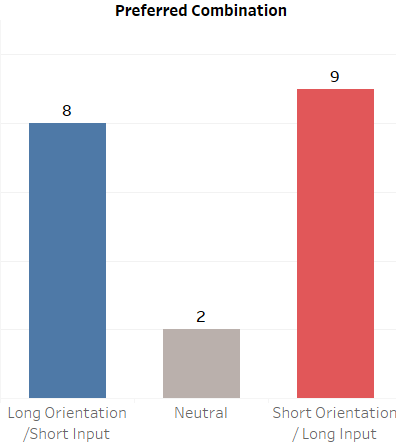
\includegraphics[width=7cm, height=9cm]{Chapters/graphics/preference.png}
\caption{A histogram, representing our participants preferences regarding the combinations.}
\label{fig:preference}
\end{figure}

As mentioned in Section \ref{4.3.2}, a form of \textit{error-recovery} was included into the application with the intention of enhancing its ease-of-use. Although the main focus of our study, was to solely examine certain ratios of \textit{orientation} and \textit{input phases}, it was interesting to find out whether the \textit{error-recovery} feature had an impact on the \textit{orientation time}. For that, a question was added to the survey which only had to be answered if a participant encountered the \textit{error recovery} during the interaction. Answers were assessed through a Likert-scale (see figure \ref{fig:survey3}, question 19). Out of 19 participants, only 6 experienced the \textit{error recovery} (see figure \ref{fig:error})\footnote{We were able to obtain this information during the study, through the database view which was incorporated in the application (see figure \ref{fig:flow}) If a participant had more than three "search-fails", it meant that they encountered the \textit{error-recovery}}. When asked whether the pop-up window feature helped them find the pattern faster, five of the concerned participants agreed and only one disagreed. Moreover, half of the concerned participants (3) disagreed that the pop-up window elongated the searching process. However, one agreed and two answered did not notice any difference. Lastly, when asked whether they found the pop-up window annoying, four disagreed, one agreed, and another was indecisive (see figure \ref{fig:error}). In order to see whether \textit{error-recovery} had an impact on the concerned participants' performance, their quantitative data was examined. Luckily, they never  encountered \textit{error-recovery} during the third level of each phase, which meant that feature had no impact of the measured time. Nonetheless, the examination of the feature's effect still provided information on whether it's design was well accepted by participants. \\


\begin{figure}[t!]
\centering
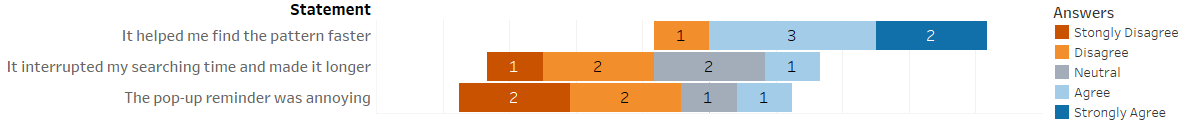
\includegraphics[width=15cm, height=3cm]{Chapters/graphics/ErrorRecovery.png}
\caption{A histogram, representing our participants preferences regarding the combinations.}
\label{fig:error}
\end{figure}







%*****************************************
\chapter{Discussion and Limitations}\label{ch:sixth}
%*****************************************

In this chapter, we will review and analyze the main results of the study (see Chapter \ref{ch:fifth}), in relation to the recommendations proposed by Zezschwitz et al. \cite{Zezschwitz} (see Section \ref{3.2.2}). Based on these results, we will discuss the universality of Zezschwitz et al.'s \cite{Zezschwitz} approach. Last, the limitations, which we faced during the design and procedure of the study, will be presented.\\

Analogous to Zezschwitz et al. \cite{Zezschwitz}, the main phases (\textit{orientation} and \textit{input}) were measured in the study. An improved approach was taken towards enhancing the accuracy of the time measurements, specifically those of \textit{orientation time}. Thus one of the limitations in Zezschwitz et al.'s \cite{Zezschwitz} approach, was the inaccuracy of the \textit{orientation time} measurements. The concept \underline{\textbf{FiPa}} was specially designed to implement Zezschwitz et al.'s \cite{Zezschwitz} measurement method, to prevent this issue. \\
Based on a further recommendation by Zezschwitz et al. \cite{Zezschwitz} the measurement of perceived efficiency was taken into consideration for the design of the study. Participants' perception of efficiency, regarding the ratios, was measured and assessed through a questionnaire. They were asked to directly compare the two main ratios \textit{short/long} and \textit{long/short} to each other, in terms of certain characteristics (mental effort, efficiency, preference, length of input, length of search, etc.). \\

Although the contrasting ratios \textit{short/long} and \textit{long/short} were designed to be asymmetrical in terms of their phase lengths\footnote{Meaning long orientation had to have the same length as long input and short orientation had to have the same length as short input.}, quantitative results have shown that, on average, their overall length differed by 1176 ms, with \textit{long/short} having the longest average duration (6056 ms). Nonetheless, apart from \textit{long/short's} the maximum orientation time (9053 ms), its remaining \textit{orientation times} did not exceed 5202 ms. In reference to the \textit{orientation times} of \textit{short/long}, this means that the "long phases" of both ratios did not differ substantially, and that their worst-case measurements were similar. The same is true for the maximum times of the "short phases" in both ratios: "short input" (in \textit{long/short}) and "short orientation" (in \textit{short/long}) barely differed by 8 ms. This shows that the design of the concept and the implementation of the ratios were suitable and successful for the purpose of this study, as in their worst cases they can be considered almost equally efficient, in terms of their measured efficiency. \\

In terms of perceived efficiency, participants were first asked to evaluate the \textbf{mental} and \textbf{practical tasks} of each ratio, separately. They were asked to rate the annoyance of a ratio's \textit{orientation} and the simplicity to memorize, as well as input its corresponding pattern. Surprisingly the memorization and input of the short and long patterns, were considered easy to memorize and input, by all participants, on average. However, the difference between both ratios was notable regarding the annoyance of their \textit{orientation times}. While, on average, all participants disagreed that \textit{short orientation} was annoying, the average opinion regarding the annoyance of \textit{long orientation} was "neutral". Even if participants did not strongly incline towards a positive or negative opinion regarding the annoyance of \textit{long orientation}, the results show a greater acceptance of \textit{short orientation}.\\

As mentioned earlier, participants were asked to compare both ratios, based on certain characteristics. The majority of the participants (68\%) found that \textit{long/short} required more mental effort than \textit{short/long} (only 16\%). This implies that, although both ratios contained a complicated task\footnote{The "long phases" of each ratio were meant to represent complicated tasks.}, complicated \textbf{mental tasks} seem to have stressed participants more than complicated \textbf{practical tasks}. Consequently, most participants (79\%) agreed that the implementation of \textit{short/long} was easier than \textit{long/short} (only 16\%). In addition, when participants were asked which of both ratios took longer to find and enter, the results indicated that participants were more sensitive towards the complexity of long \textit{orientation phases} than they were towards \textit{long input phases}. While all participants (100\%) agreed that the pattern in \textit{long/short} took longer to find than in \textit{short/long}, only 74\% agreed that it took longer to enter in \textit{short/long} and the rest (26\%) saw no difference. Participants' incline towards the ratio \textit{short/long} was more notable when they were asked which ratio implementation they found more efficient. The majority leaned towards \textit{short/long} and only 26\% found \textit{long/short} to be more efficient. \\

Based on these analyzed results, one might expect that, in general,  participants would have had a greater incline towards \textit{short/long} than towards \textit{long/short}. However, when asked to chose one ratio implementation as a screen lock for their smartphone, this was not the case. Although 47\% chose the ratio \textit{short/long} for their screen lock, still 42\% chose \textit{long/short}. It is clear to see that there isn't a significant difference between both percentile rates, as the only differ by 5\%. It is assumed that participants who chose \textit{long/short}, made their choice with regard to the potential security aspects of the ratio design, as the most frequently given reasons for \textit{long/short} were "more secure" and "more difficult". Nonetheless, most participants chose \textit{short/long} for their screen lock. The most frequent reasons given were "more secure", as well as "more efficient". These reasons imply a higher user-acceptance and preference for \textit{short/long}, in terms of usability. The remaining 11\% (2) did not choose either of both ratios, yet they gave interesting reasons why. One participant said that they preferred \textit{short/long}, as it is easier. Yet, because it would be less secure, they would much rather prefer a combination of both ratios for their screen lock. This implies they would favor a concept that is not only easier to use, but that also assures to be secure enough to protect their smartphone. Another participant stated that it did not matter to them which one, they chose, as they would get used to either ratio, with time. They added that the choice would depend, more specifically on one's mood. This opinion indicates that, for some, the usability of a concept is not only dependent of its design and implementation, yet could also be determined by the user himself and by the specific needs and preferences they might have in a particular situation. \\

To see whether there was a correlation between participants' ratio preferences and their personal screen lock choice, they were asked to share the type of authentication mechanism which they used and the length or complexity of their secret. It was assumed that participants who used short and simple secrets, would choose \textit{short/long}, and the ones who used longer secrets would choose the latter. In comparing both sets of information, no notable behavioral pattern was noted. \\

All in all, the conducted study has shown that by "measuring all stages" \cite{Zezschwitz}, it was possible to receive a more accurate conception of the ratios' measured performance. Combined with "measuring perceived speed" \cite{Zezschwitz} qualitatively, participants' perceptions and opinion appeared more comprehensible and justifiable during the evaluation. By comparing participants' perception on the implementation of \textit{long/short} and \textit{short/long}, it was noticeable that the majority of participants favored the concept design, where \textit{orientation time} did not exceed \textit{input time}. Although \textit{long/short} had an simple \textbf{practical task}, results showed that it did not compensate for complicated \textbf{mental task} which it presented. This validates previous observations in the project that \textit{orientation time} should be kept low for better user-acceptance. The fact that more participants found \textit{long orientation} to be longer than \textit{long input}, validates that phase ratios should be "in favor" of the input phase . This shows that users are less bothered by the required effort for accomplishing a complicated \textbf{practical tasks}, than they are of complicated \textbf{mental tasks}. Especially when mental tasks are randomized, as each one represents a unique challenge, which can not be simplified over time through the strength of muscle memory (as with memorizing long secrets). In the concept \underline{\textbf{FiPa}}, each grid differed from the other in all ratio implementations, yet the factor of randomization was more noticeable for \textit{long/short}, as the \textit{traps}, which were uniquely set, complicated the search process even more. This is also a reason why participants had a stronger incline towards the orientation of \textit{short/long}. Therefore, randomization should truly be avoided or minimized, as suggested by Zezschwitz et al. \cite{Zezschwitz}. \\


\section{Limitations}

Although \underline{\textbf{FiPa}} was designed to emulate an authentication process, to help participants adjust to the context of the study more easily, it is not clear whether their evaluation of the ratios might have differed if the they had interacted with the concept in real-life scenarios\footnote{Meaning if the participants had used the implementation of the concept as an authentication mechanism for a certain period of time (similar to the study design of Zezschwitz et al. \cite{Zezschwitz}).}. As the concept was only used for a short period of time, there is a chance that participants' preferences and the study results might have differed.\\

Unfortunately, the study had to be conducted twice. The first study involved a wider and more versatile demographic, however, its quantitative results were not usable, by cause of an error in the implementation of the time measurements of the application. Sadly, the error was detected, afterwards, during the evaluation of the results. Consequently, an additional study had to be conducted and a new set of participants had to be recruited because the former participants were already familiar with the contents of the study and would have caused a bias in the results. The majority of the newly recruited participants were computer science students, as they had to be collected on short notice. This is another reason why the results of this study cannot be fully generalized, as most of the participants had an IT-background and were also familiar with the importance of smartphone security. The outcome of the study would have been more interesting and convincing, if the participants had a wider demographic and did not use screen locks on their smartphone. In combination with a longitude study, it would have been possible to obtain more detailed information on the perceived efficiency and the user-acceptance of the main ratios, represented in the concept. As mentioned in Chapter \ref{ch:second}, the primary reason why smartphone users persist not to use a screen lock is due to their perceived inconvenience. It would have been interesting to find out, which of the ratio implementation had the potential of motivating users to use authentication mechanisms on their smartphone and improve their smartphone security behavior. Depending on their preference regarding the ratios it would have been possible to derive the true effect of \textit{orientation time} and perceived efficiency. As a result a standard could be developed, to guarantee a enhanced user-acceptance and a higher perceived efficiency for future authentication concept propositions.

In the study, the questionnaire included a semantic differential with the intent to evaluate the aesthetics of the application. The intention was to examine how participants perceived the aesthetics of the application and to see whether their performance and preference was positively or negatively influenced by it. However, during the evaluation it was noted that these observations would exceed the scope of this thesis and distract from its true focus, namely the effect of orientation time on the perceived efficiency of authentication mechanisms.  


%*****************************************
\chapter{Conclusion and Future Work}\label{ch:seventh}
%*****************************************
\bibliographystyle{plain}
\bibliography{FrontBackmatter/Bibliography}
%\include{multiToC} % <--- just debug stuff, ignore for your documents
% ********************************************************************
% Backmatter
%*******************************************************
\appendix
%\cleardoublepage\part{Appendix}
%*******************************************************
% Appendix - CBF algorithm
%*******************************************************
\chapter{Appendix}\label{ch:appendix}

%********************************************************************
% Other Stuff in the Back
%*******************************************************
\cleardoublepage

%\cleardoublepage\pagestyle{empty}

\hfill

\vfill


\pdfbookmark[0]{Colophon}{colophon}
\section*{Colophon}
This thesis was typeset with \LaTeXe\ using Hermann Zapf's
\emph{Palatino}
and \emph{Euler} type faces (Type~1 PostScript fonts \emph{URW
Palladio L}
and \emph{FPL} were used). The listings are typeset in \emph{Bera
Mono}, originally developed by Bitstream, Inc. as ``Bitstream Vera''.
(Type~1 PostScript fonts were made available by Malte Rosenau and
Ulrich Dirr.)

The typographic style was inspired by \cauthor{bringhurst:2002}'s genius as
presented in \emph{The Elements of Typographic Style} 
\citep{bringhurst:2002}. It is available for \LaTeX\ via \textsmaller{CTAN} as 
``\href{http://www.ctan.org/tex-archive/macros/latex/contrib/classicthesis/}%
{\texttt{classicthesis}}''.

\paragraph{note:} The custom size of the textblock was calculated
using the directions given by Mr. Bringhurst (pages 26--29 and
175/176). 10~pt Palatino needs  133.21~pt for the string
``abcdefghijklmnopqrstuvwxyz''. This yields a good line length between
24--26~pc (288--312~pt). Using a ``\emph{double square textblock}''
with a 1:2 ratio this results in a textblock of 312:624~pt (which
includes the headline in this design). A good alternative would be the
``\emph{golden section textblock}'' with a ratio of 1:1.62, here
312:505.44~pt. For comparison, \texttt{DIV9} of the \texttt{typearea}
package results in a line length of 389~pt (32.4~pc), which is by far
too long. However, this information will only be of interest for
hardcore pseudo-typographers like me.%

To make your own calculations, use the following commands and look up
the corresponding lengths in the book:
\begin{verbatim}
    \settowidth{\abcd}{abcdefghijklmnopqrstuvwxyz}
    \the\abcd\ % prints the value of the length
\end{verbatim}
Please see the file \texttt{classicthesis.sty} for some precalculated 
values for Palatino and Minion.

    \settowidth{\abcd}{abcdefghijklmnopqrstuvwxyz}
    \the\abcd\ % prints the value of the length


\bigskip

\noindent\finalVersionString




% ********************************************************************
% Game Over: Restore, Restart, or Quit?
%*******************************************************
\end{document}
% ********************************************************************
